\documentclass{beamer}

\usepackage{graphicx}
\usepackage[normalem]{ulem}
\usepackage{tikz}

\definecolor{arrowcolor}{rgb}{0.5,0.5,1}

\mode<presentation>{
  \usetheme{Warsaw}
}
\title{Git Deep Dive}
\subtitle{How Distributed Version Control Can Save Your Life}
\author{Josh Larson}

\begin{document}

\AtBeginSection[]{
  \begin{frame}
    \tableofcontents[
      currentsection,
      sectionstyle=show/shaded,
      subsectionstyle=hide/hide/hide
    ]
  \end{frame}
  \begin{frame}
    \tableofcontents[
      currentsection,
      sectionstyle=show/hide,
      subsectionstyle=show/show/hide
    ]
  \end{frame}
}

\titlepage

\section{Why Version Control?}

\begin{frame}
  \newcommand{\photosize}{0.6\textwidth}

  \frametitle{Photo Syncing}

  \begin{columns}
    \begin{column}{0.35\textwidth}
      \begin{center}
        \textbf{Server}
        \begin{figure}[l]  
          \uncover<1-6,8->{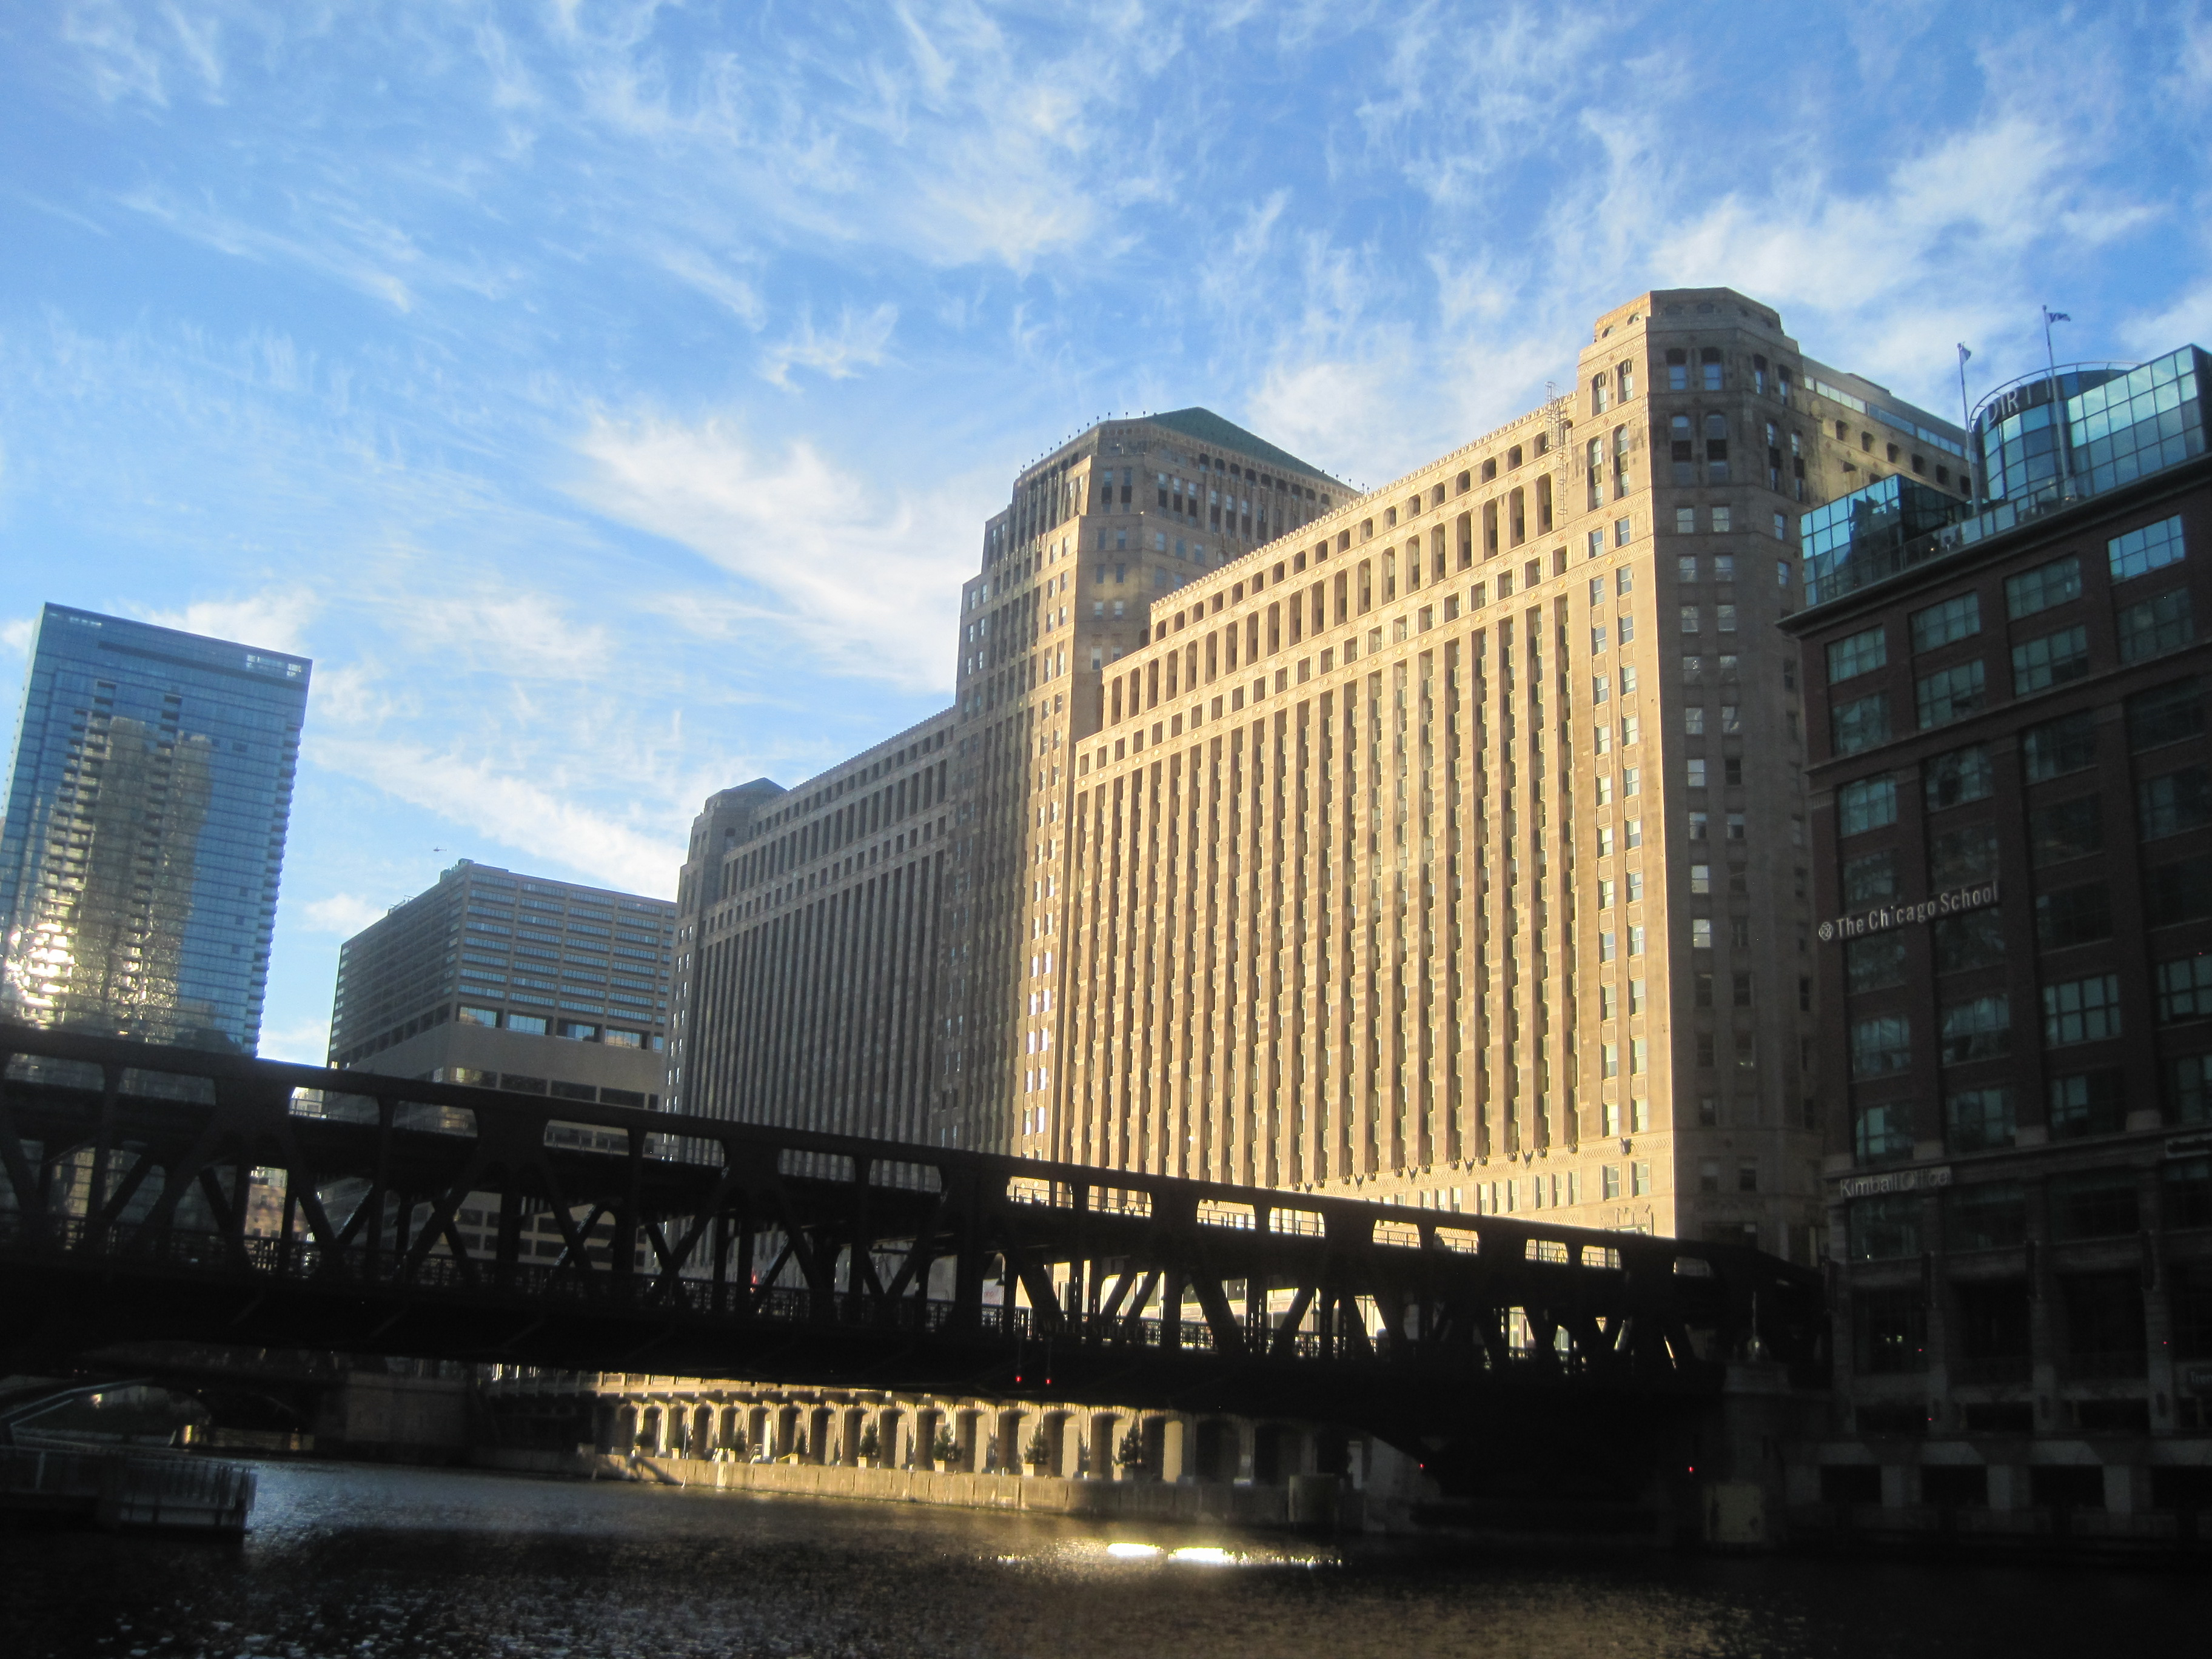
\includegraphics[width=\photosize]{merchmart}}

          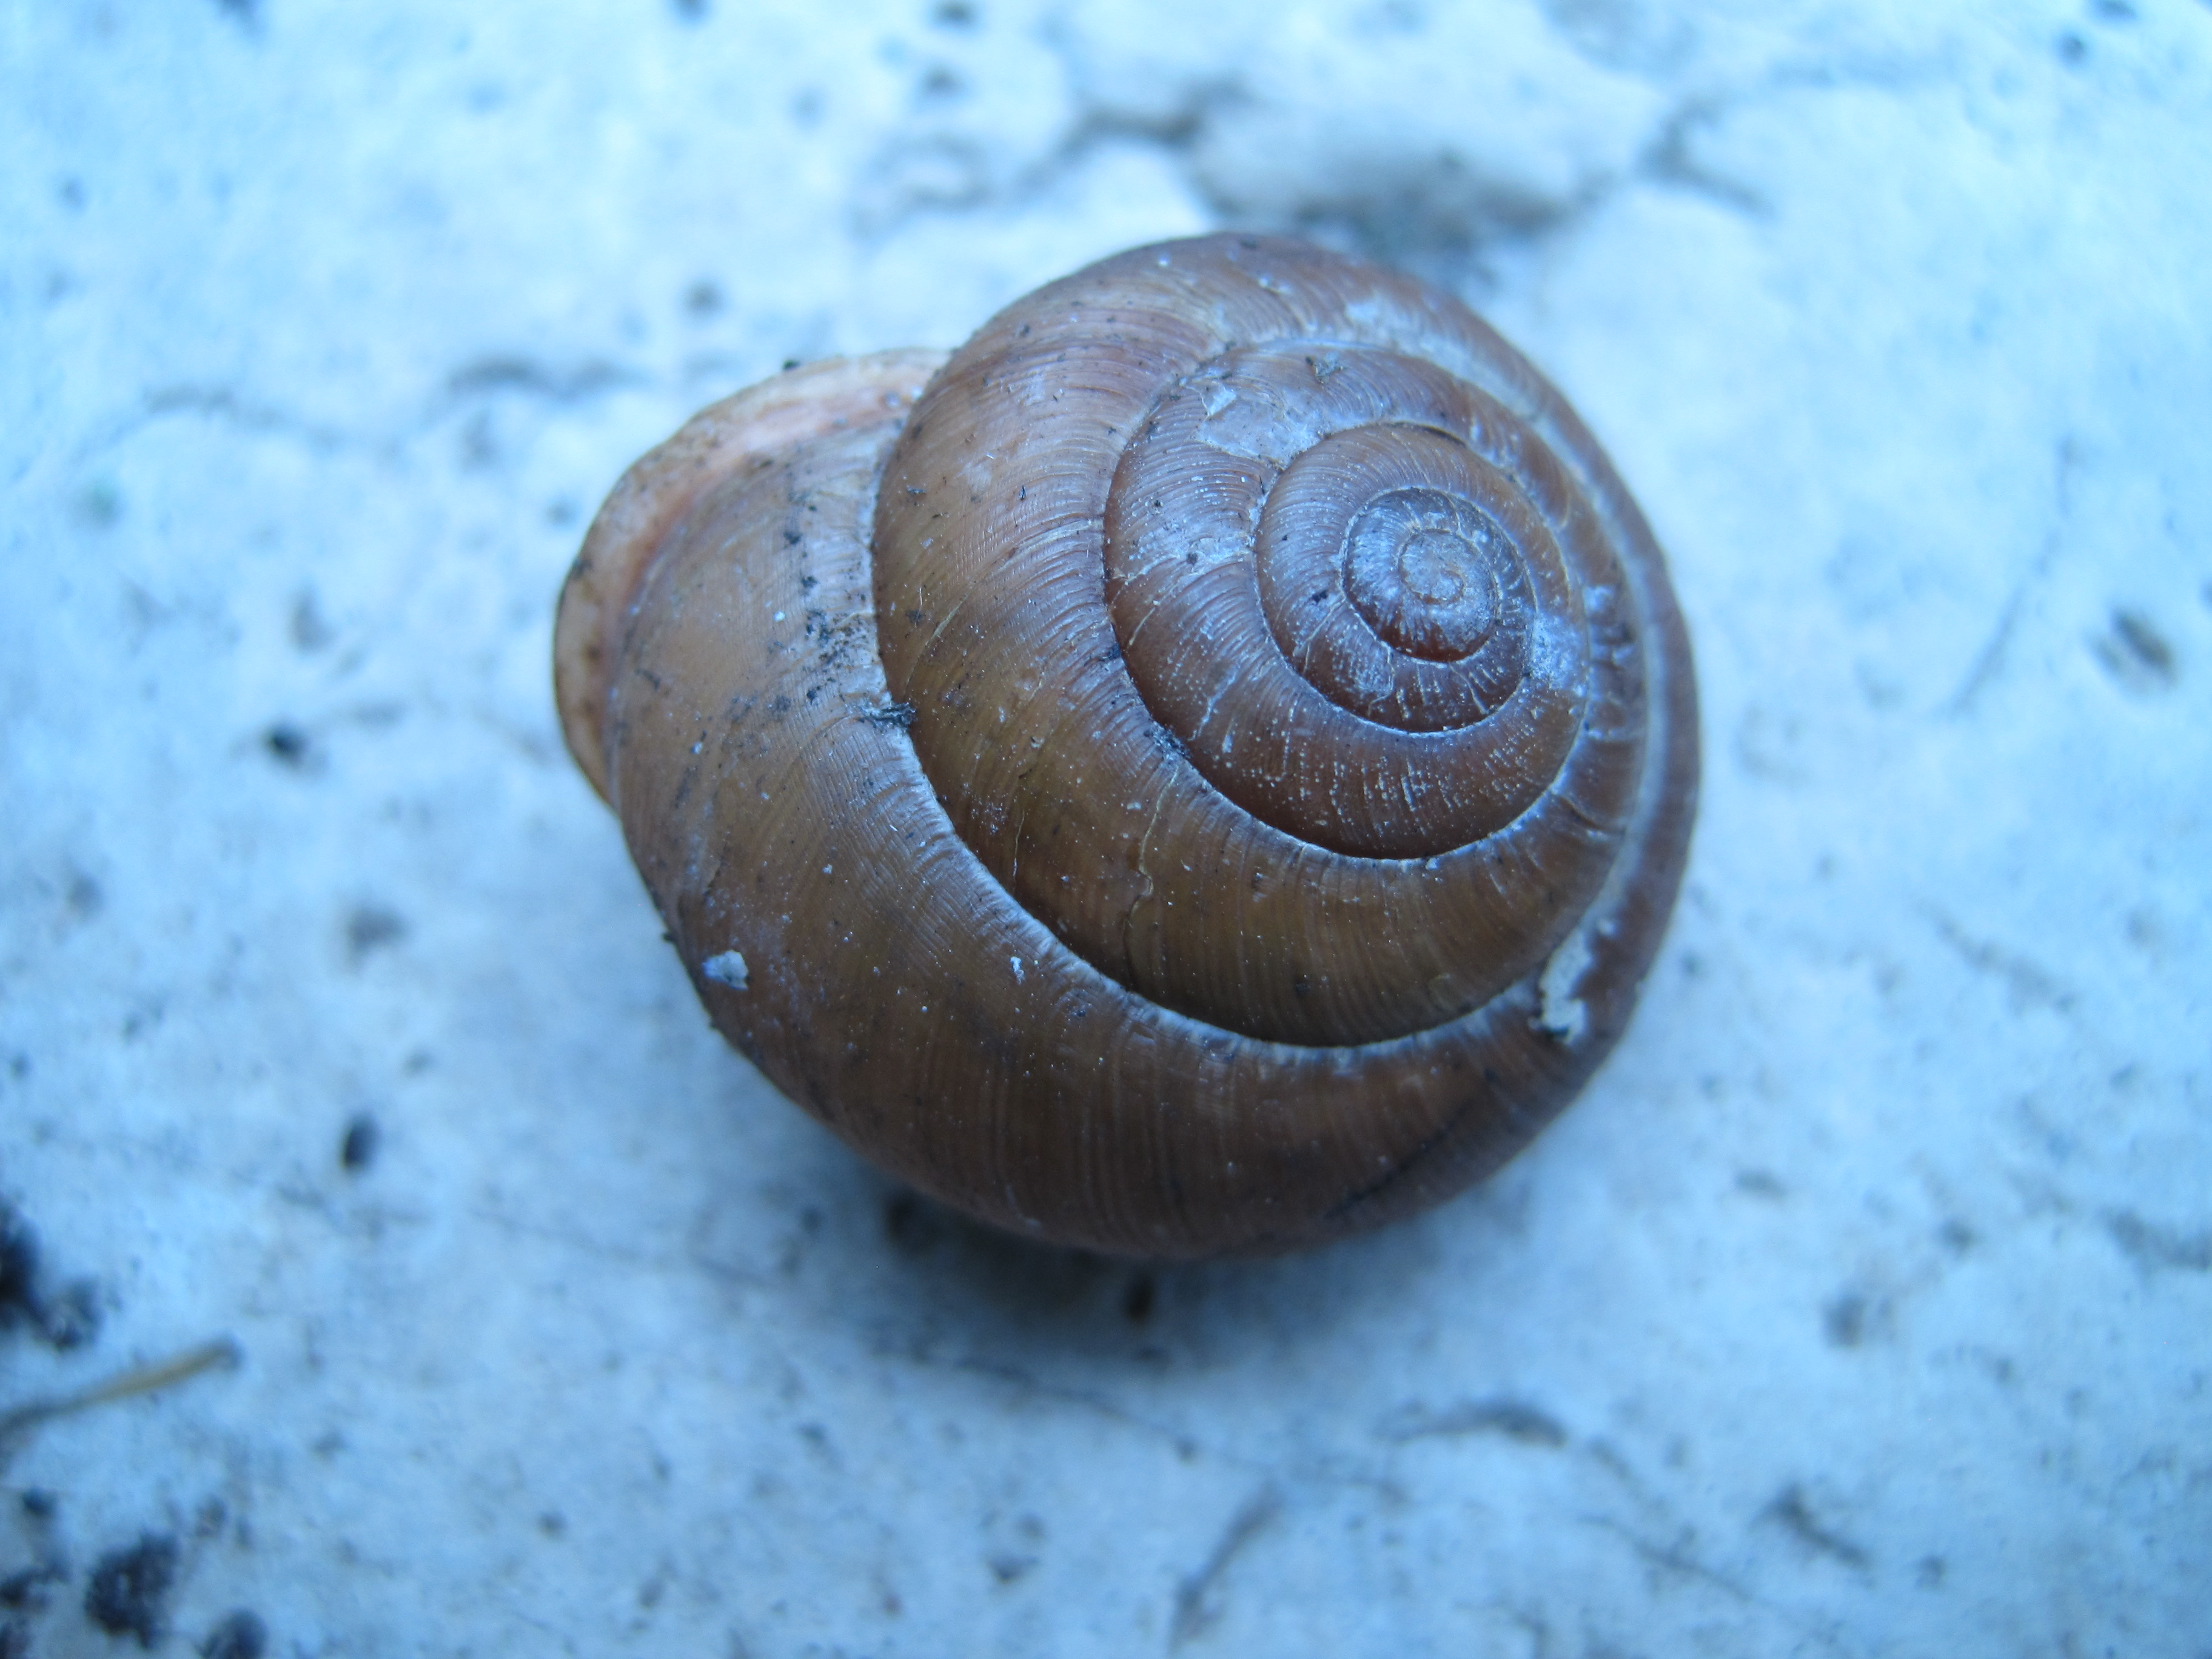
\includegraphics[width=\photosize]{shell}

          \uncover<4->{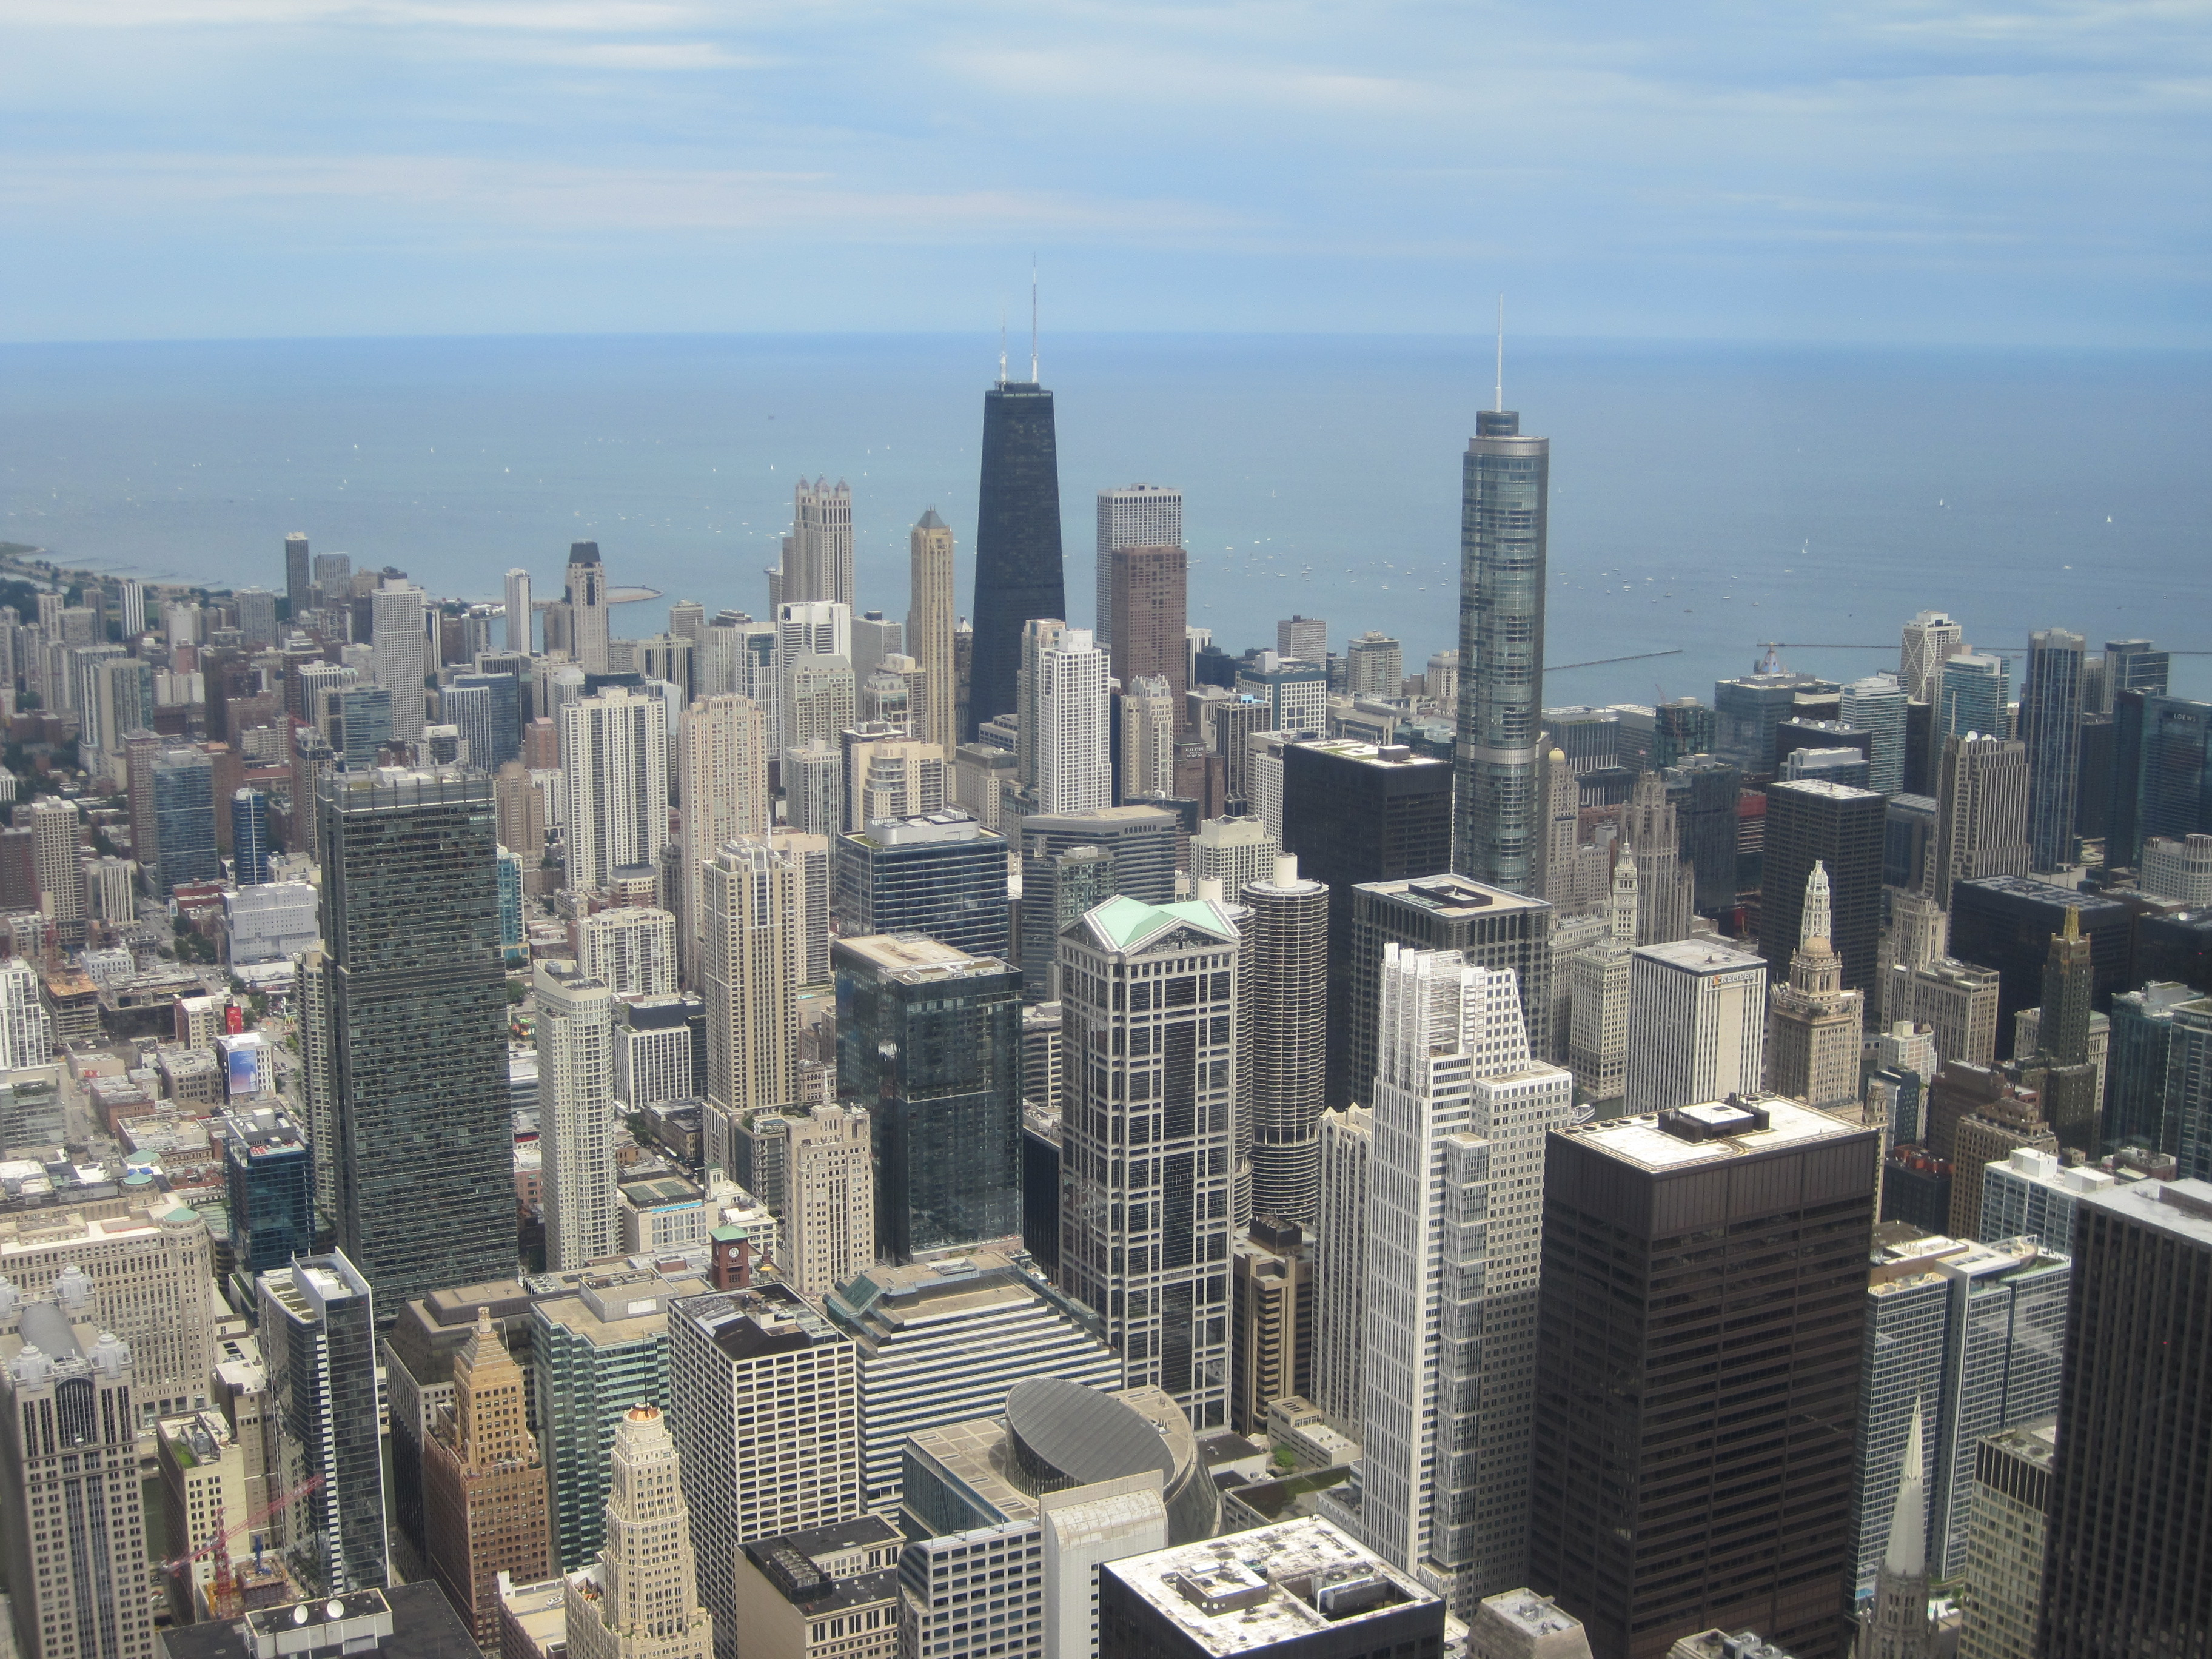
\includegraphics[width=\photosize]{skyline}}
        \end{figure}
      \end{center}
    \end{column}

    \begin{column}{0.3\textwidth}
      \begin{center}
        \uncover<2->{
          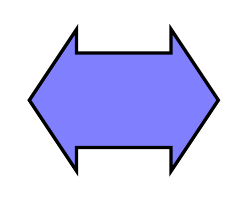
\begin{tikzpicture}[scale=0.3, fill=arrowcolor, draw=black, very thick]
            \filldraw
            (-2,2) --
            (2,2) --
            (2,3) --
            (4,0) --
            (2,-3) --
            (2,-2) --
            (-2,-2) --
            (-2,-3) --
            (-4,0) --
            (-2,3) --
            cycle;
          \end{tikzpicture}
        }
      \end{center}
    \end{column}
    
    \begin{column}{0.35\textwidth}
      \begin{center}
        \textbf{Laptop}
        \begin{figure}
          \uncover<3-5,9->{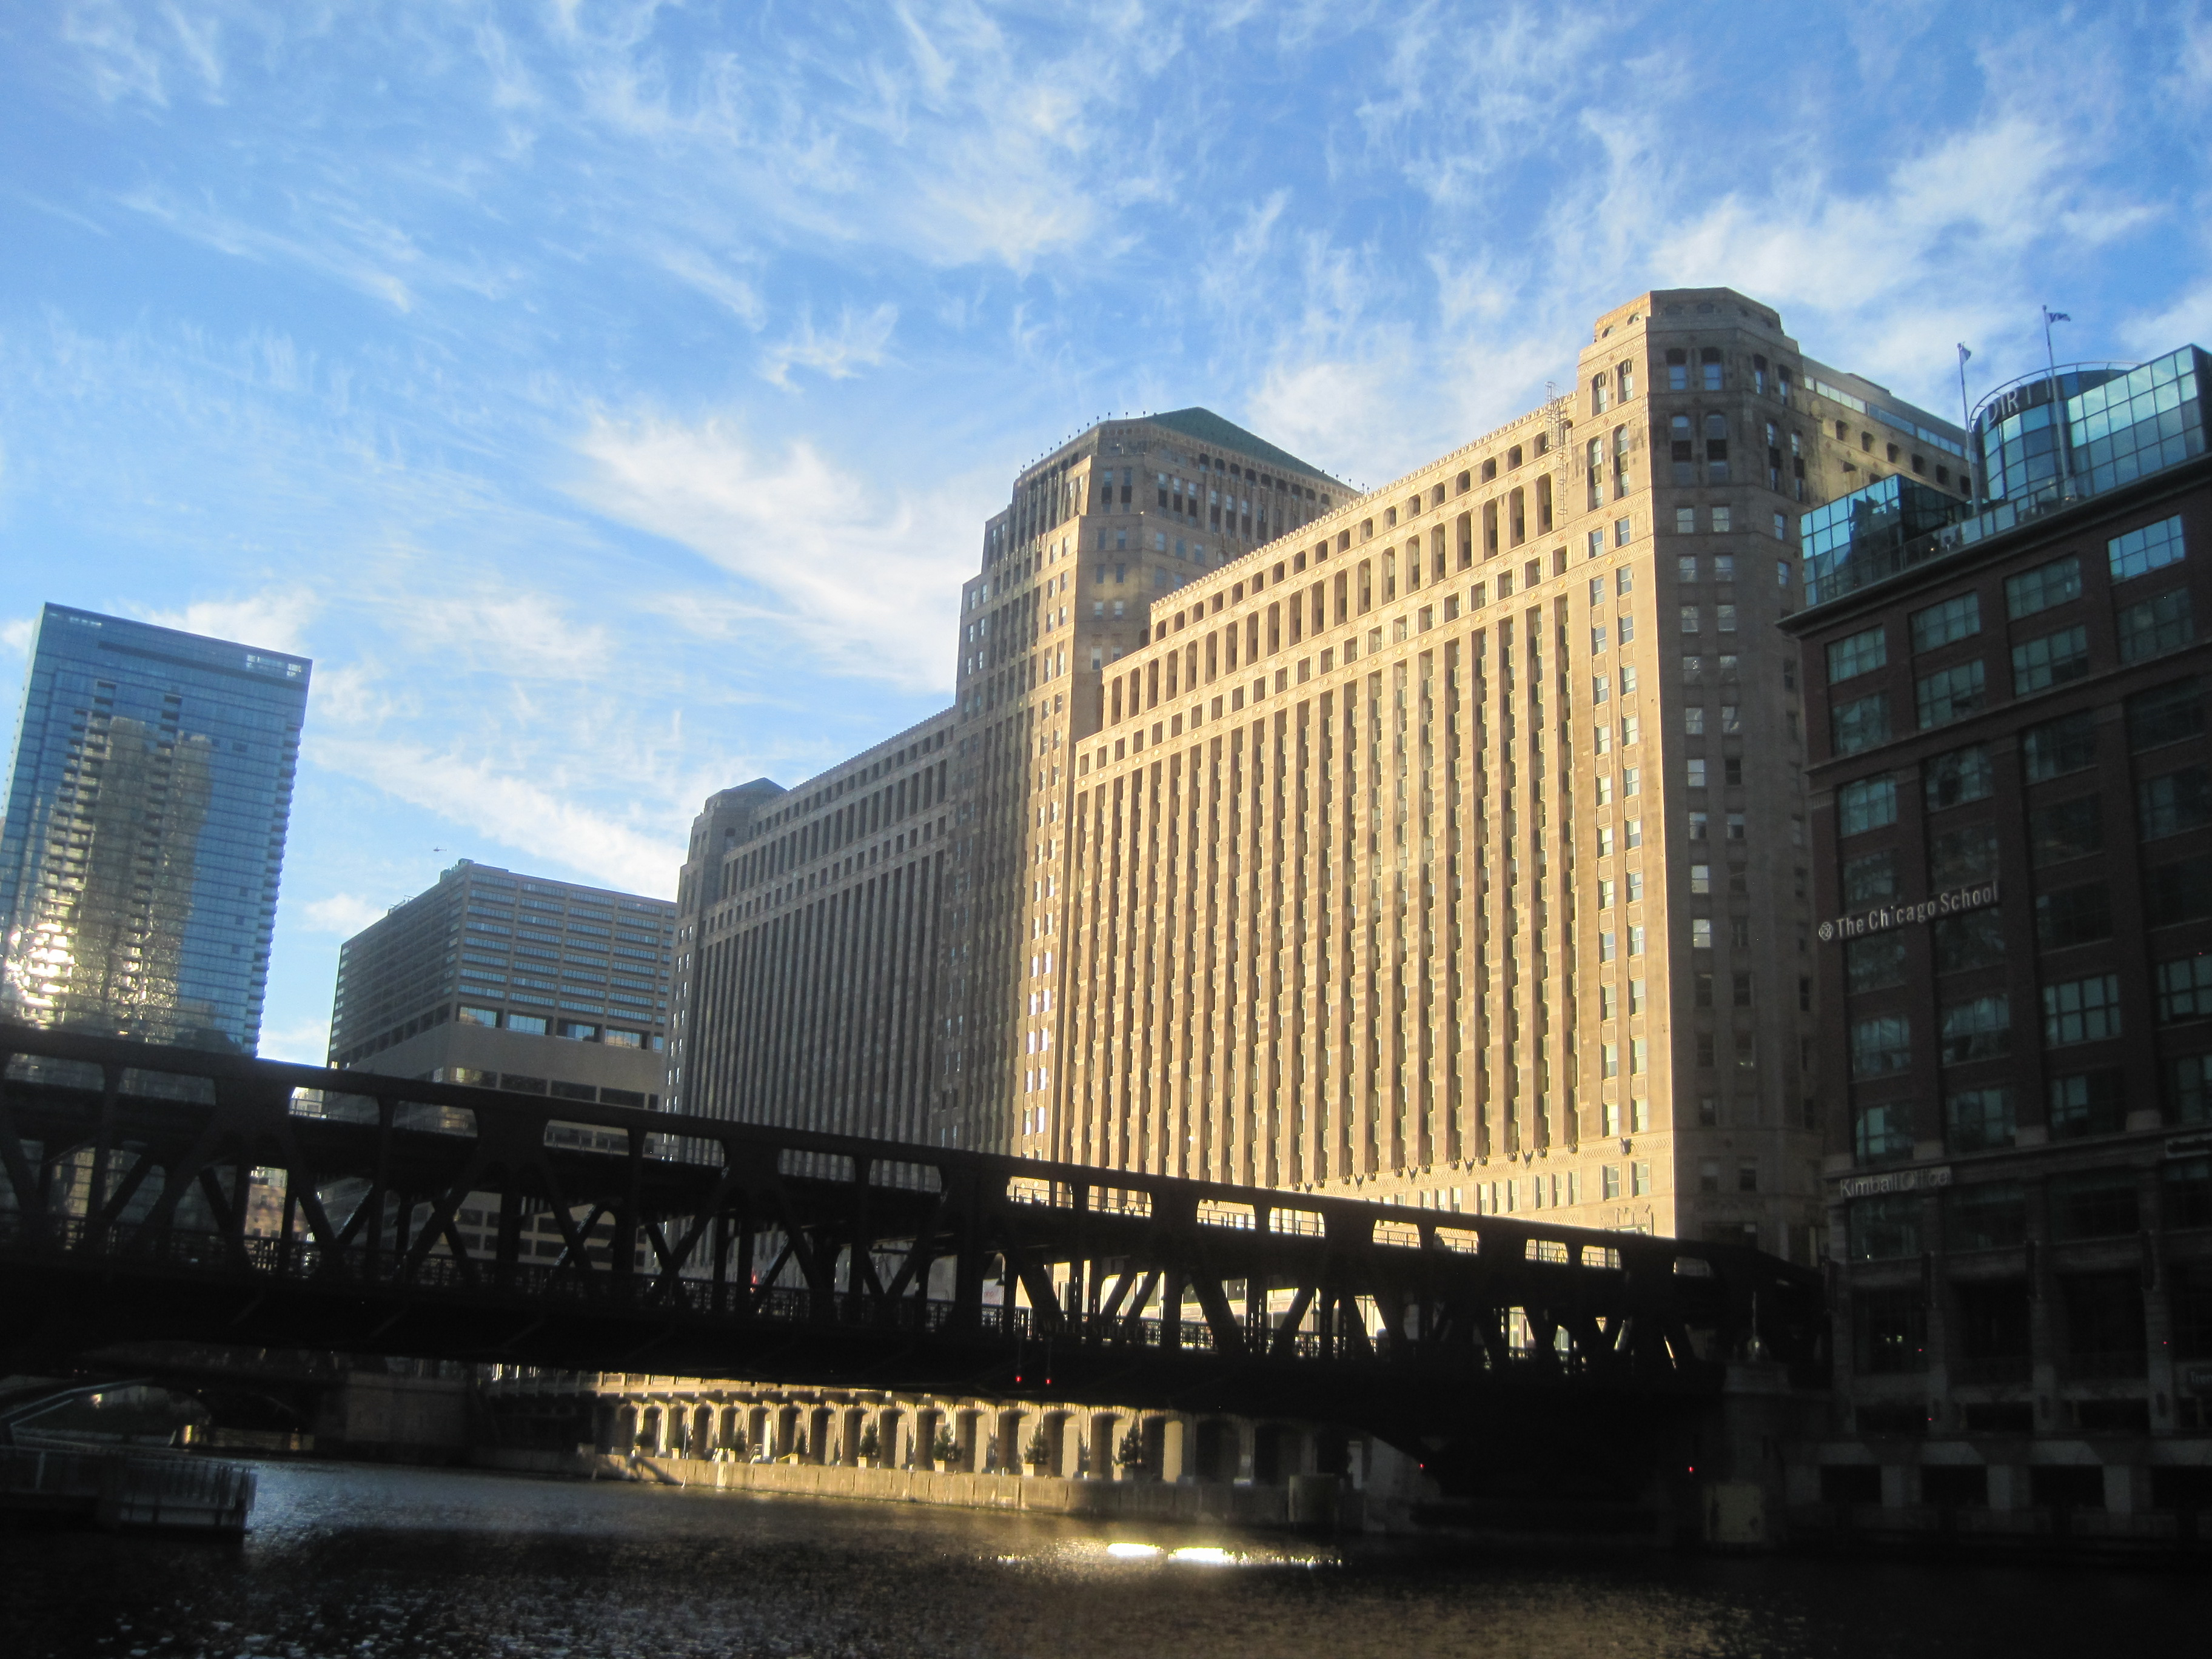
\includegraphics[width=\photosize]{merchmart}}

          \uncover<3->{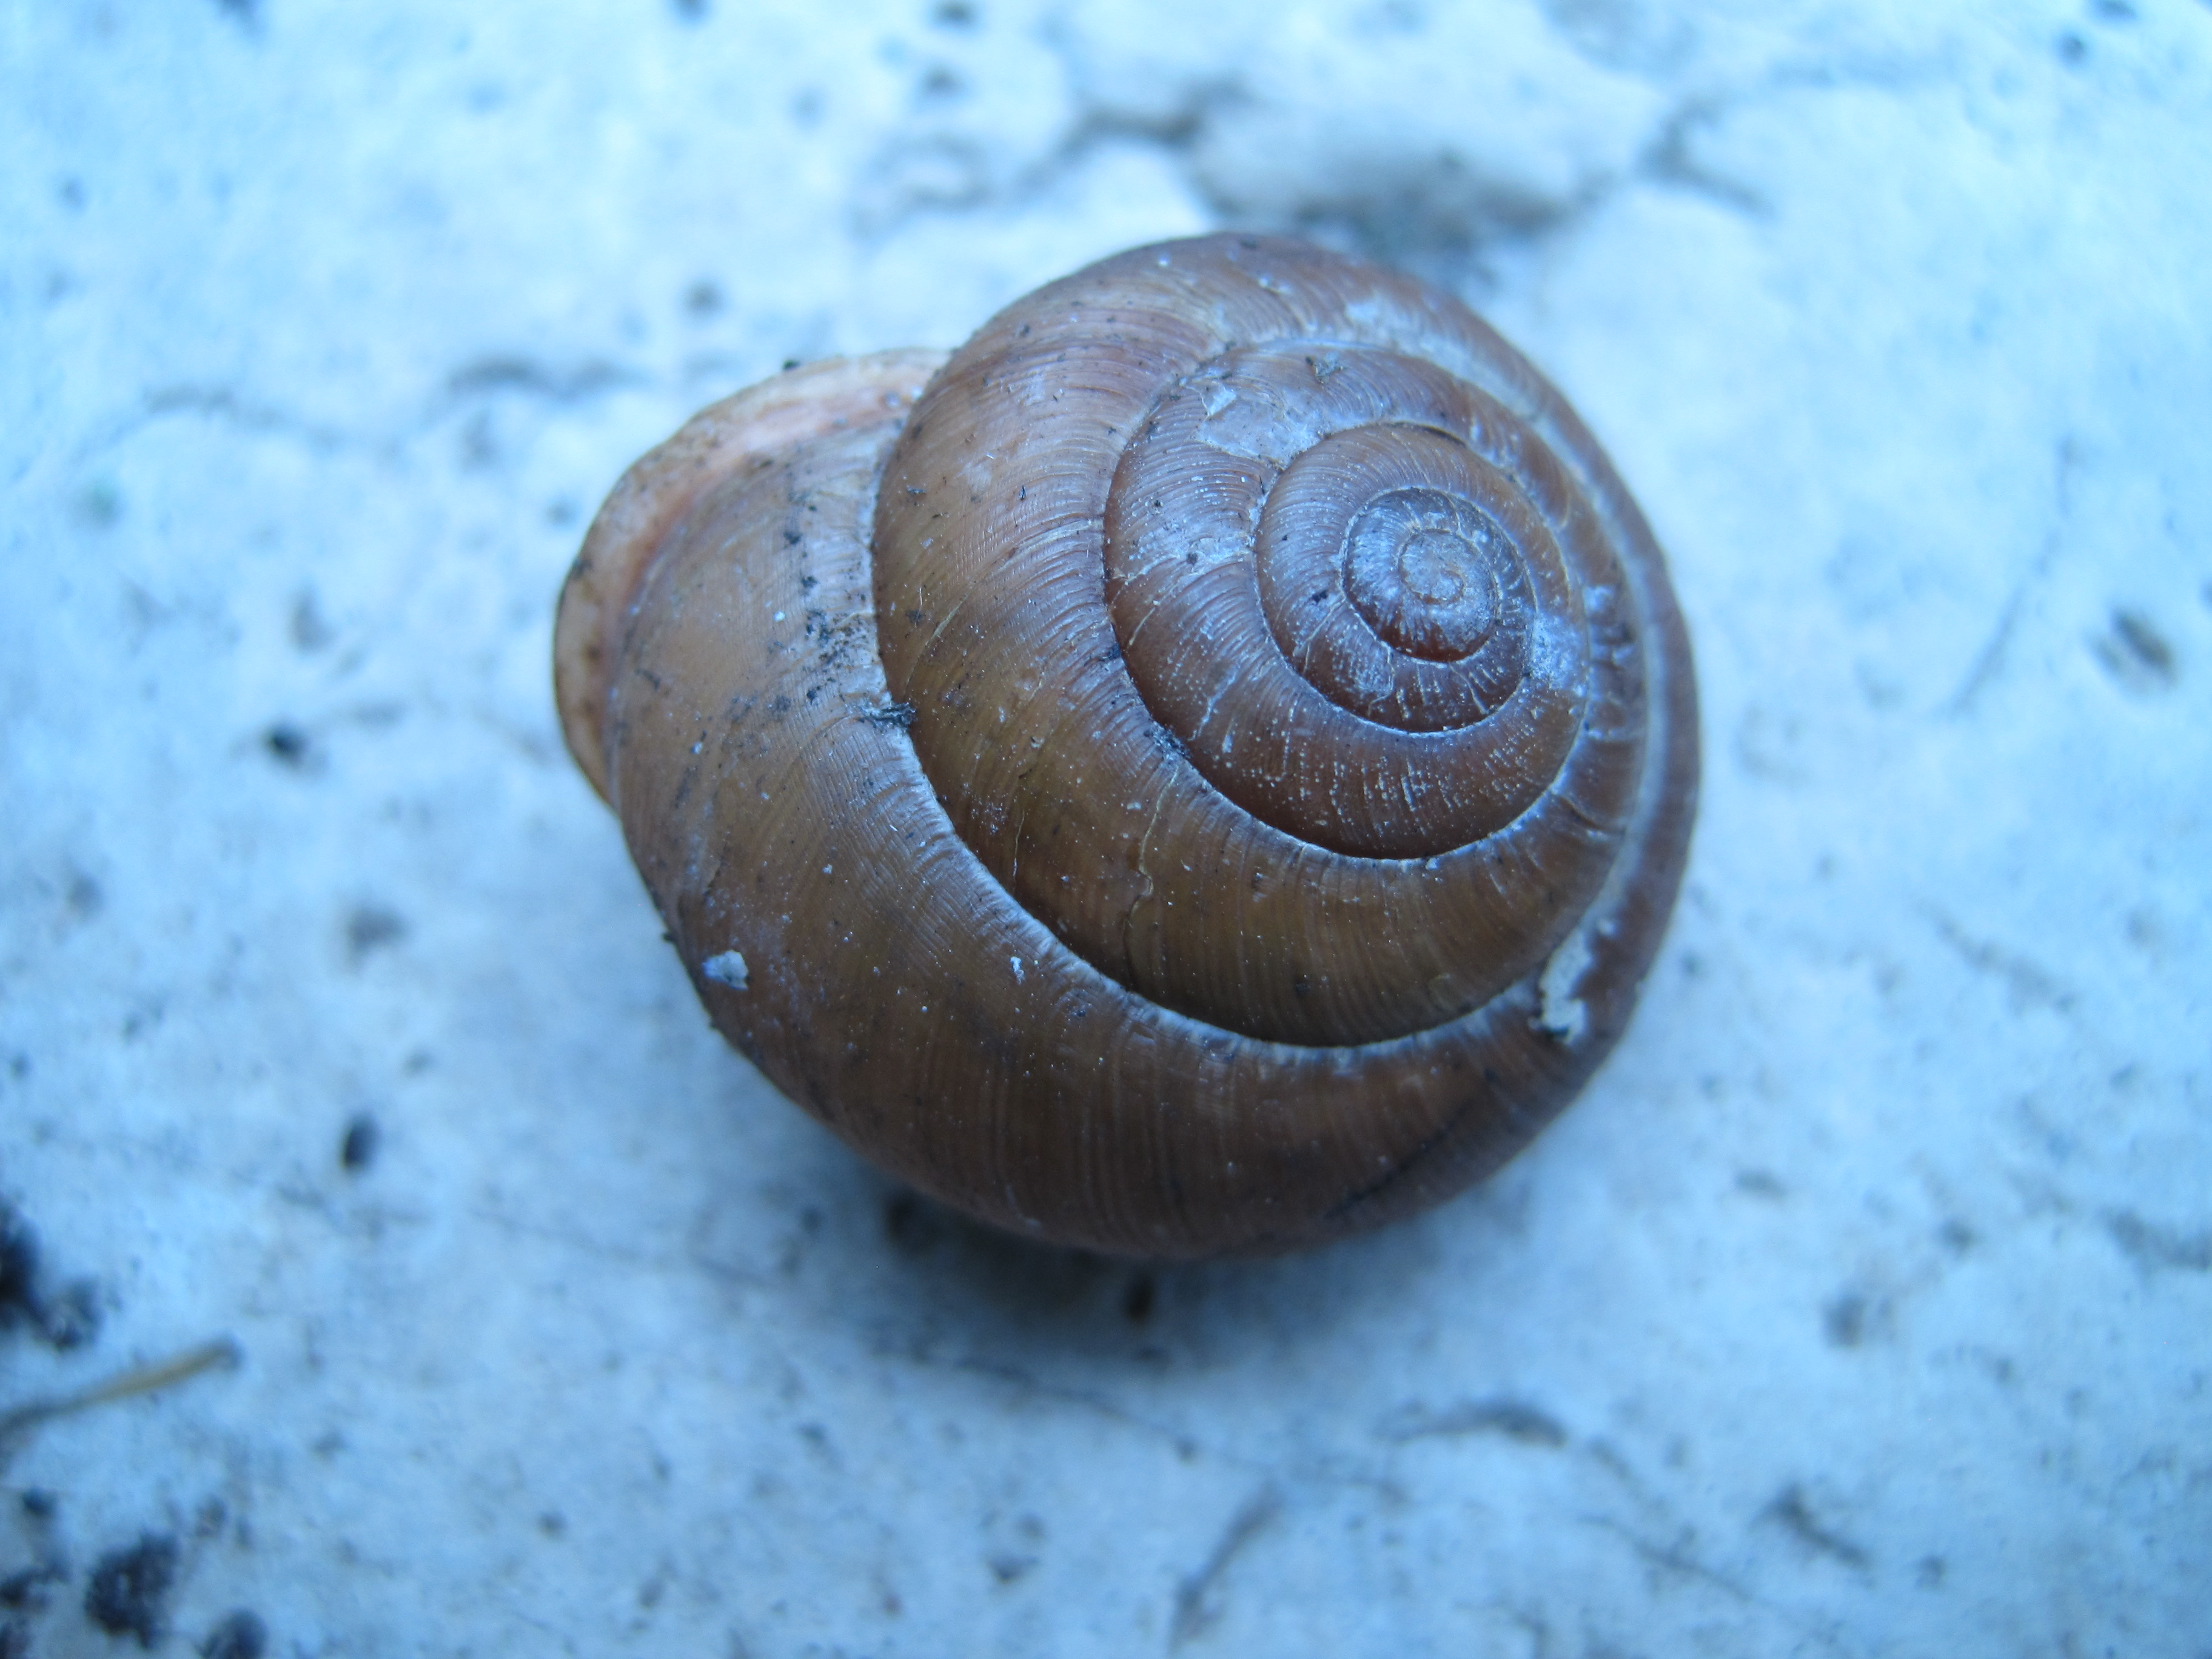
\includegraphics[width=\photosize]{shell}}

          \uncover<5->{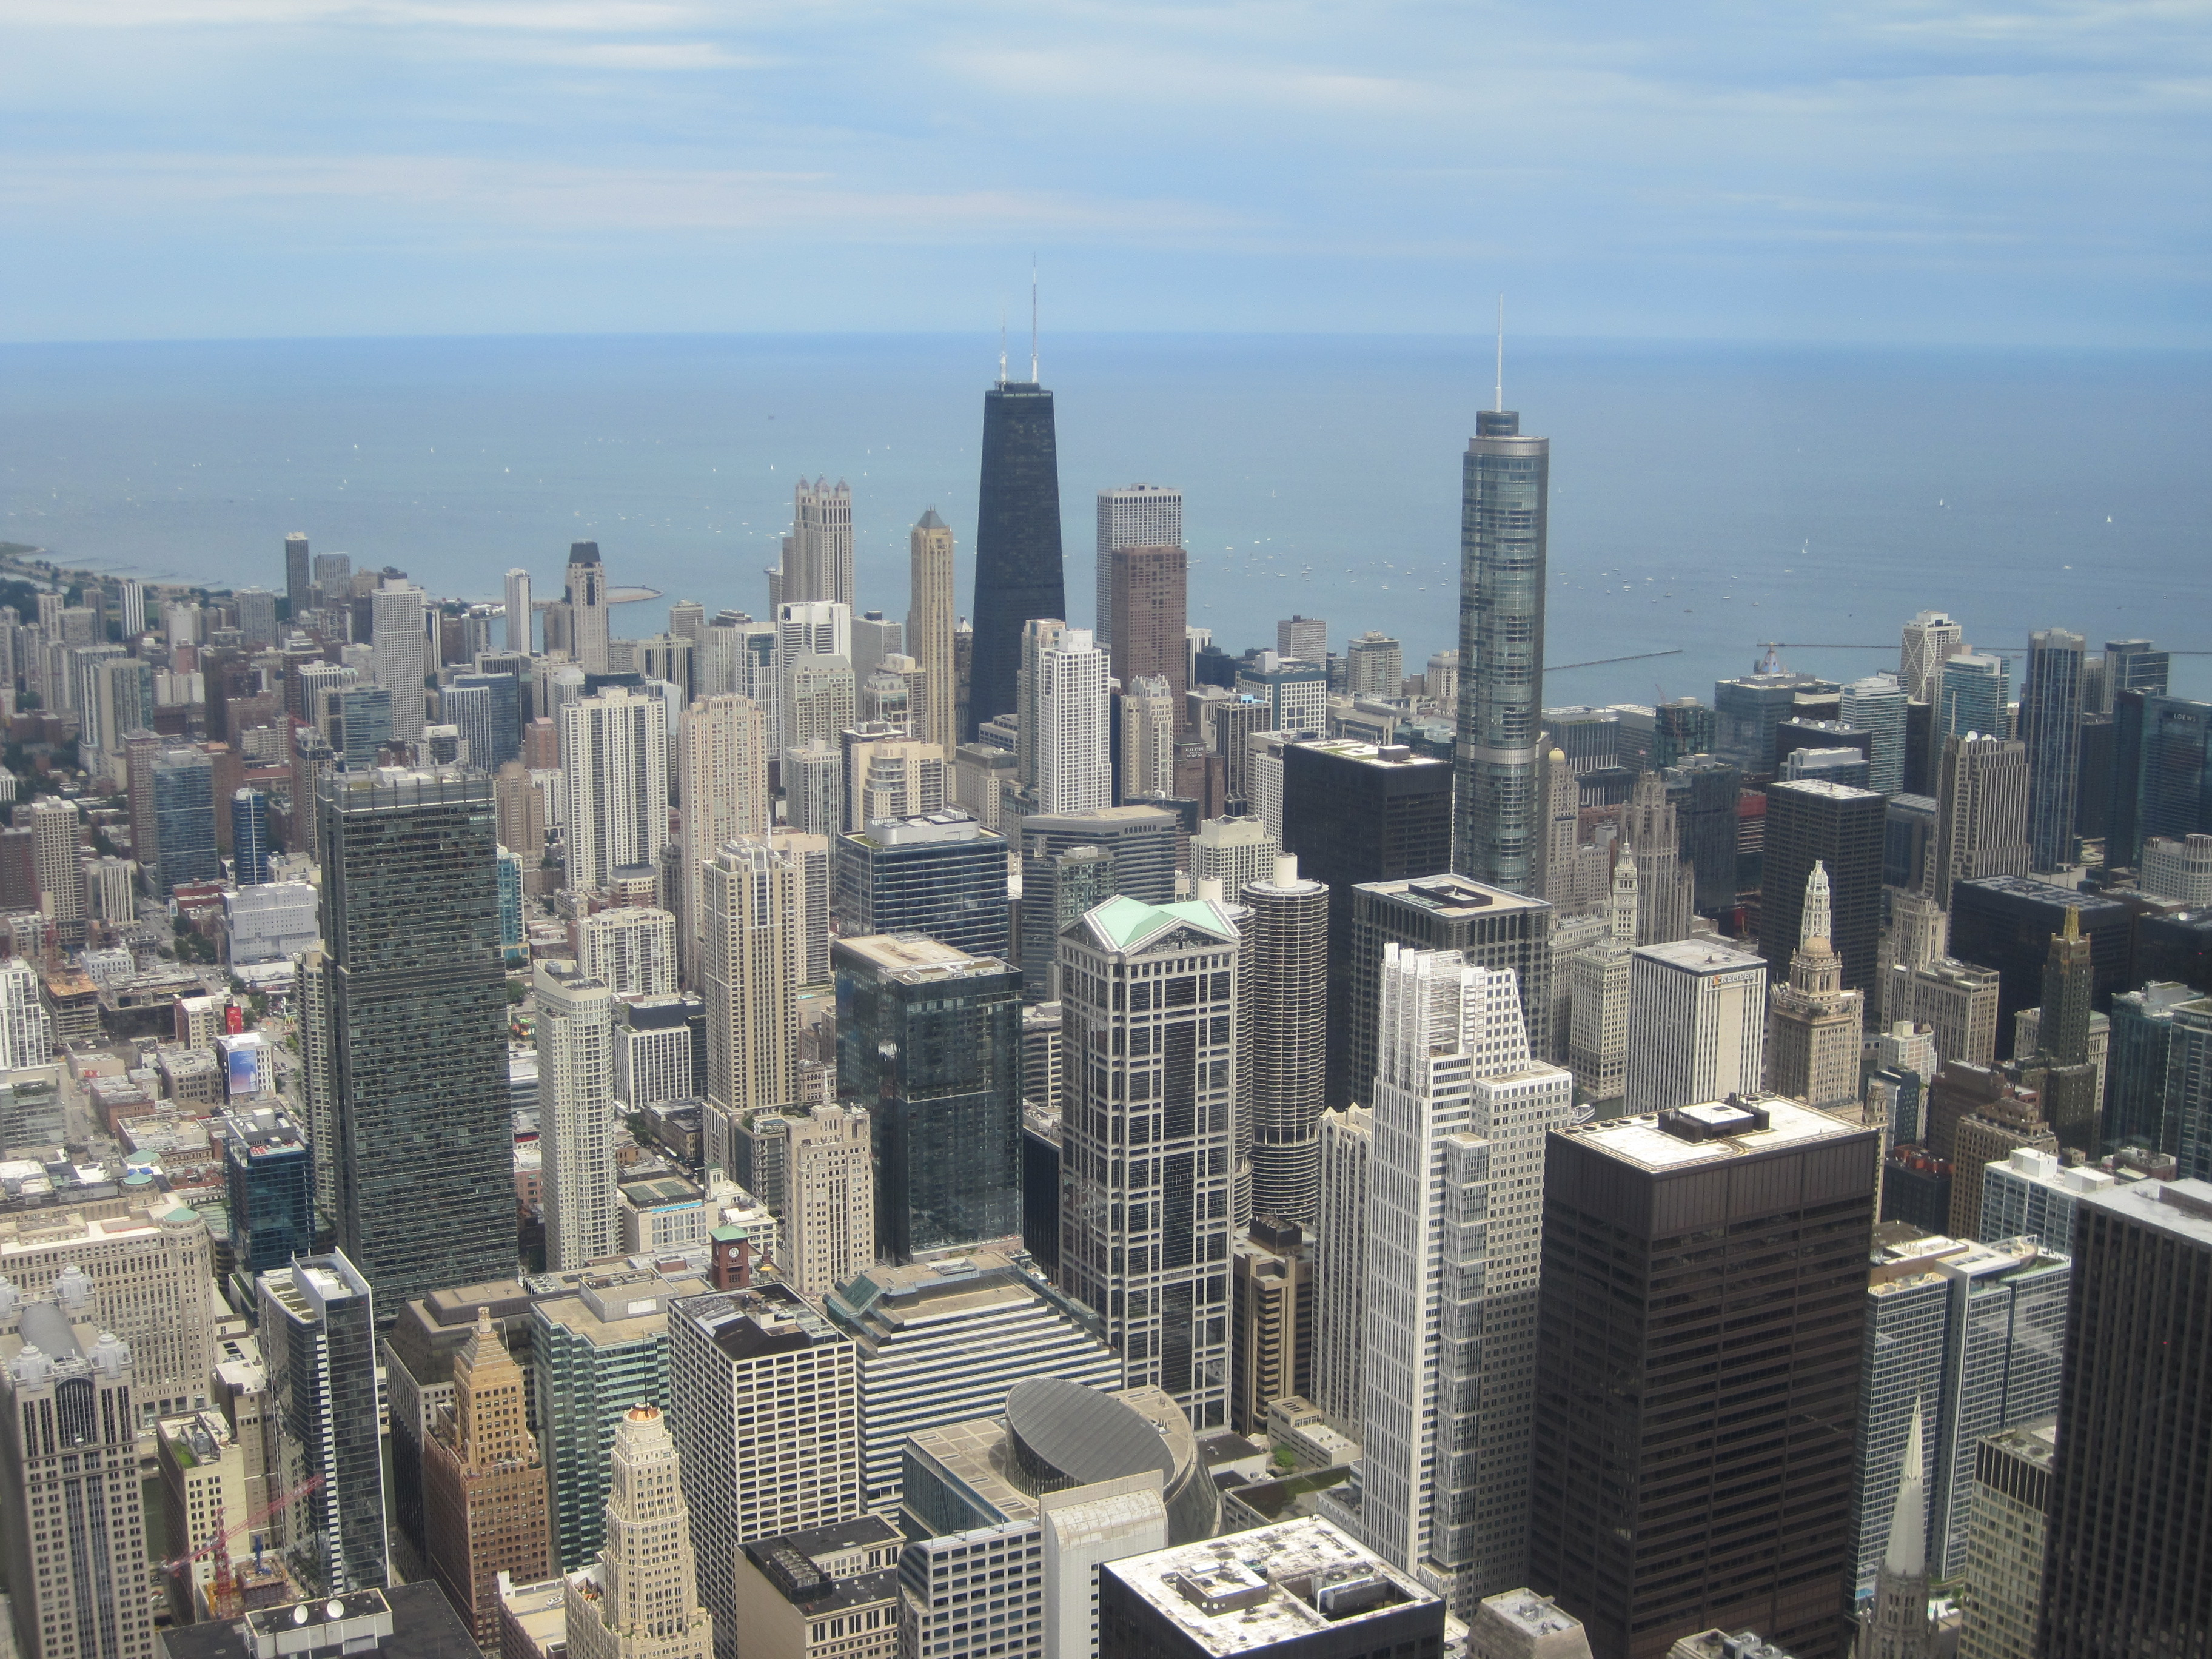
\includegraphics[width=\photosize]{skyline}}
        \end{figure}
      \end{center}
    \end{column}
  \end{columns}
\end{frame}

\begin{frame}
  \frametitle{Photo Versions}

  \begin{itemize}
    \pause
  \item State of the World
    \begin{itemize}
      \pause
    \item Image is present on the server
      \pause
    \item ...and not the client
    \end{itemize}
    \pause
  \item Does this mean ``Added to server; should add to client''
    \pause
  \item ...or ``Deleted from client; should delete from server''
  \end{itemize}
\end{frame}

\begin{frame}
  There's no way to tell.
  \pause
  Not with the information we have now.
\end{frame}

\begin{frame}
  \newcommand{\photosize}{0.5\textwidth}

  \frametitle{Photo Versions}

  \begin{columns}
    \begin{column}{0.5\textwidth}
      \begin{itemize}
      \item Instead of snapshots, \uncover<2->{keep track of \textit{changes}}
        \begin{itemize}
        \item<3-> Add \texttt{merchmart} and \texttt{shell}
        \item<5-> Add \texttt{skyline}
        \item<7-> Remove \texttt{merchmart}
        \end{itemize}
      \end{itemize}
    \end{column}

    \begin{column}{0.5\textwidth}
      \begin{center}
        \uncover<4-7>{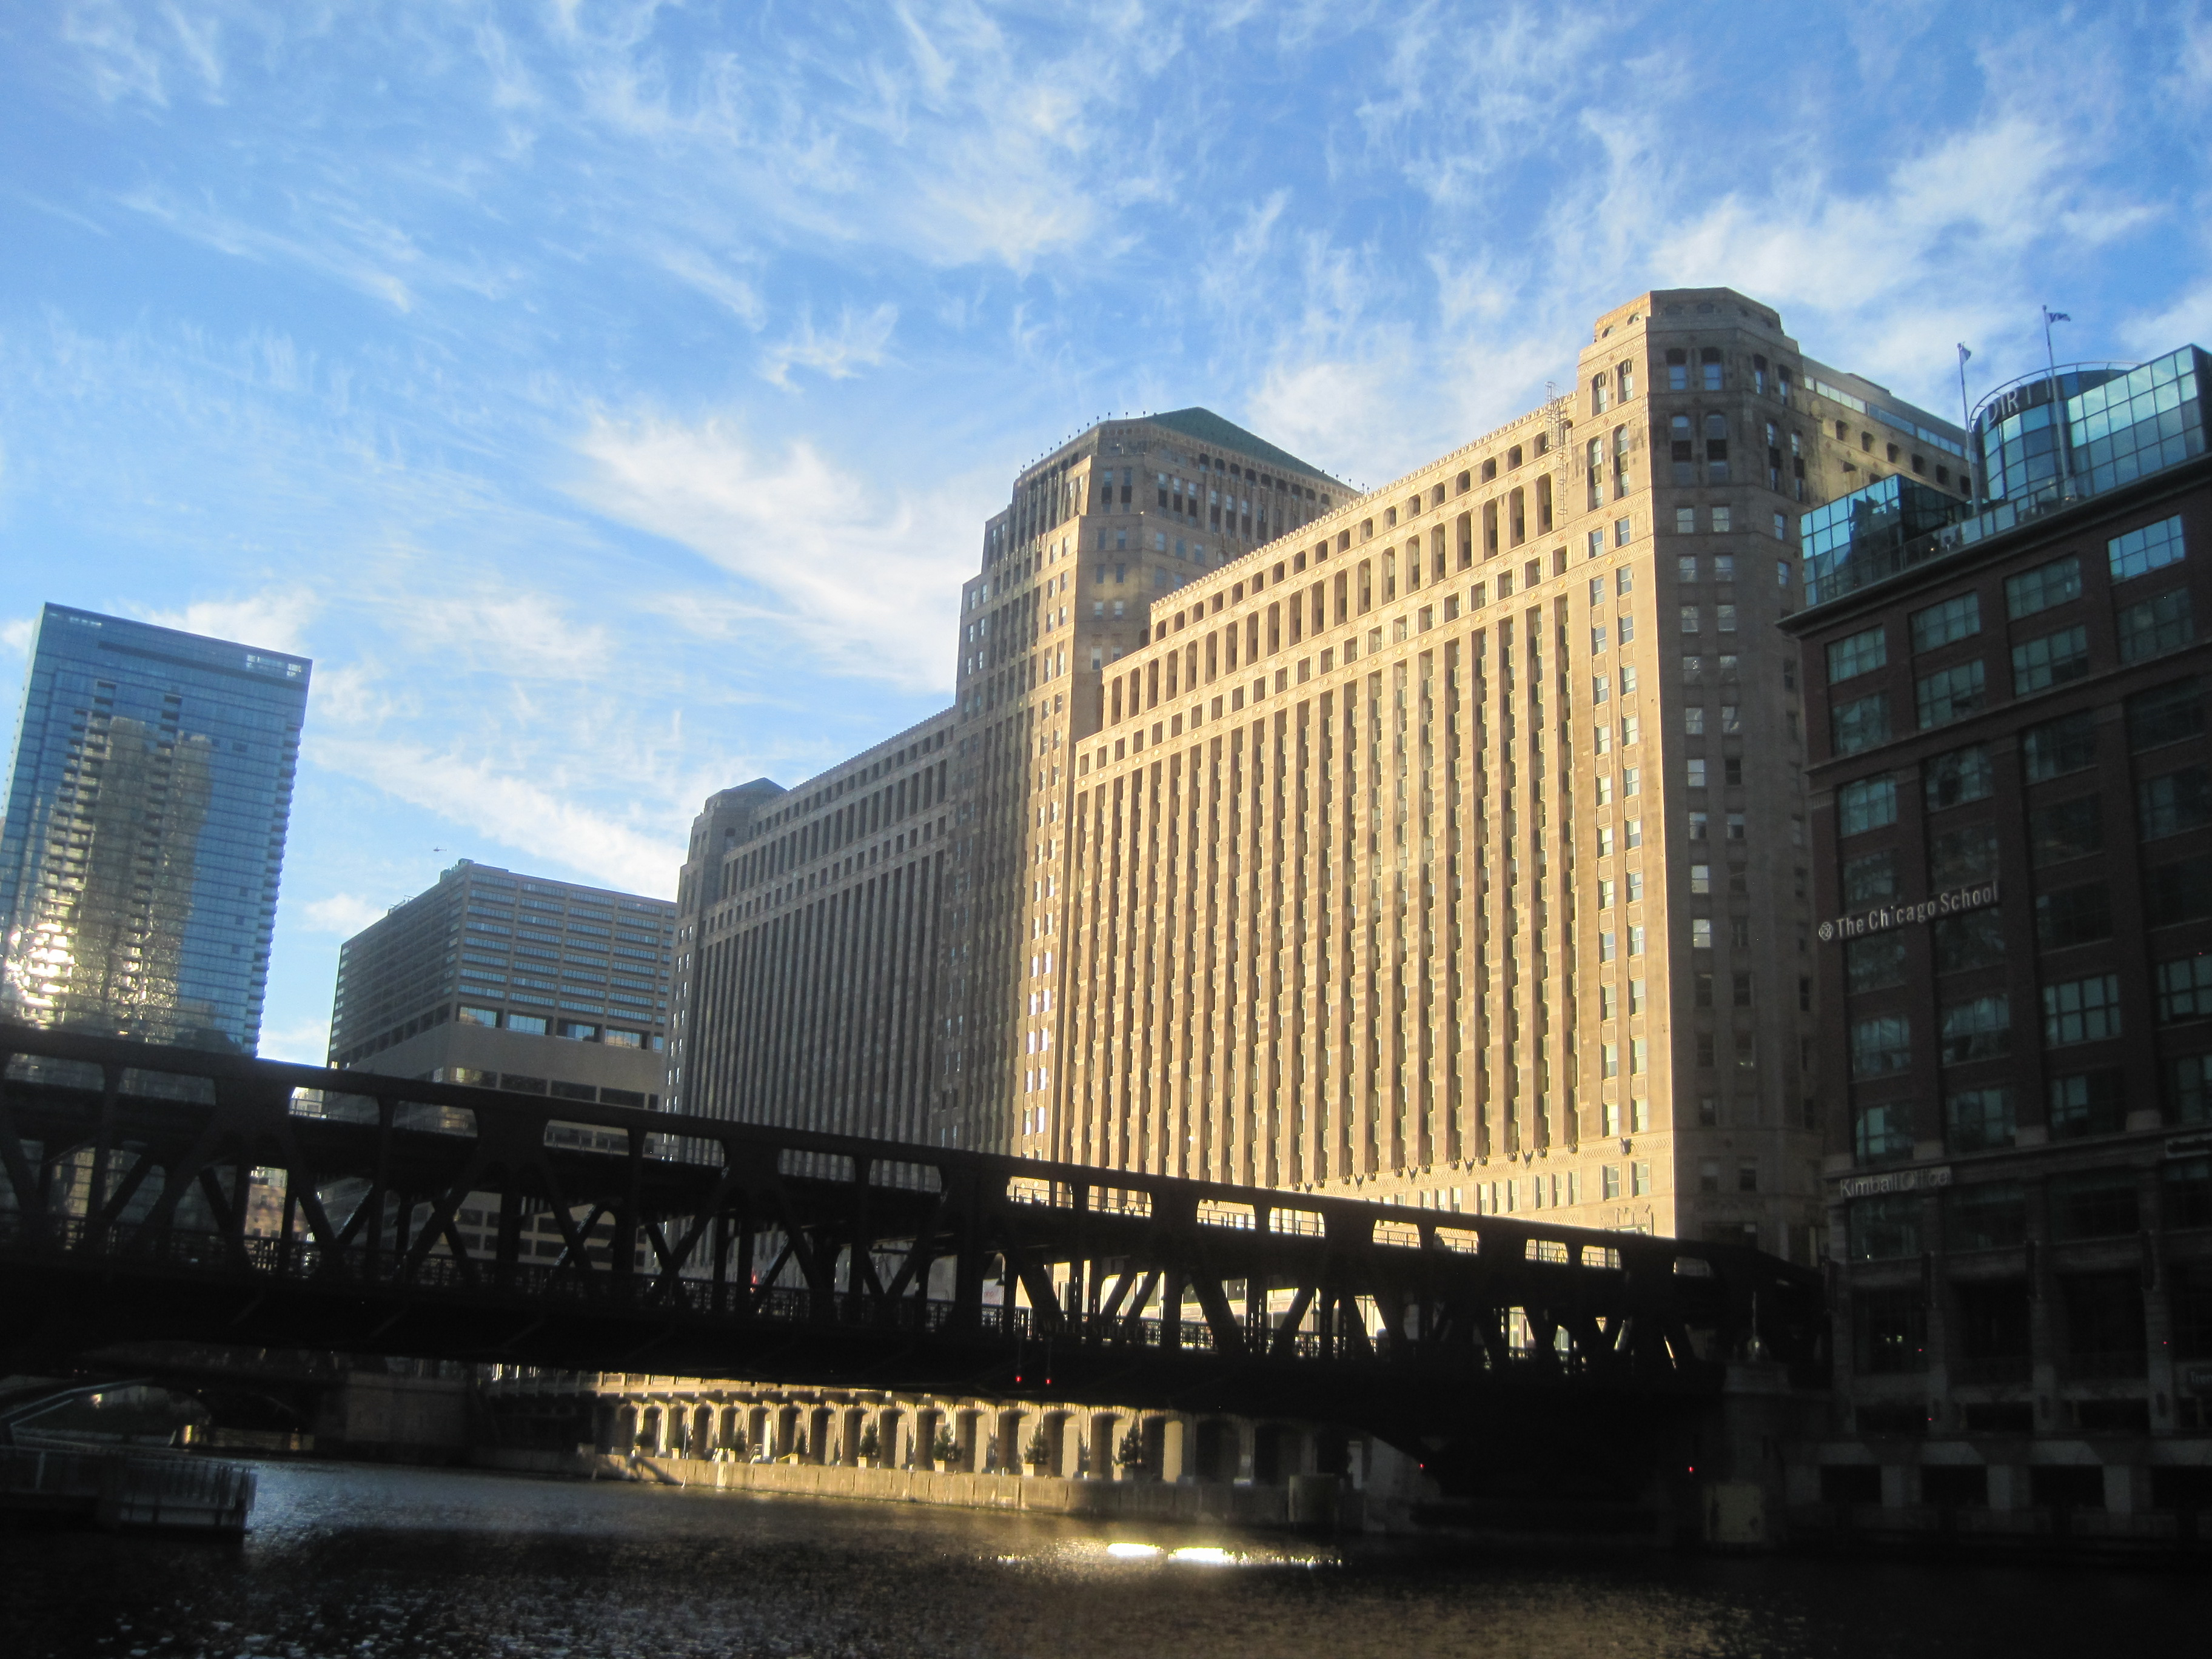
\includegraphics[width=\photosize]{merchmart}}
        
        \uncover<4-8>{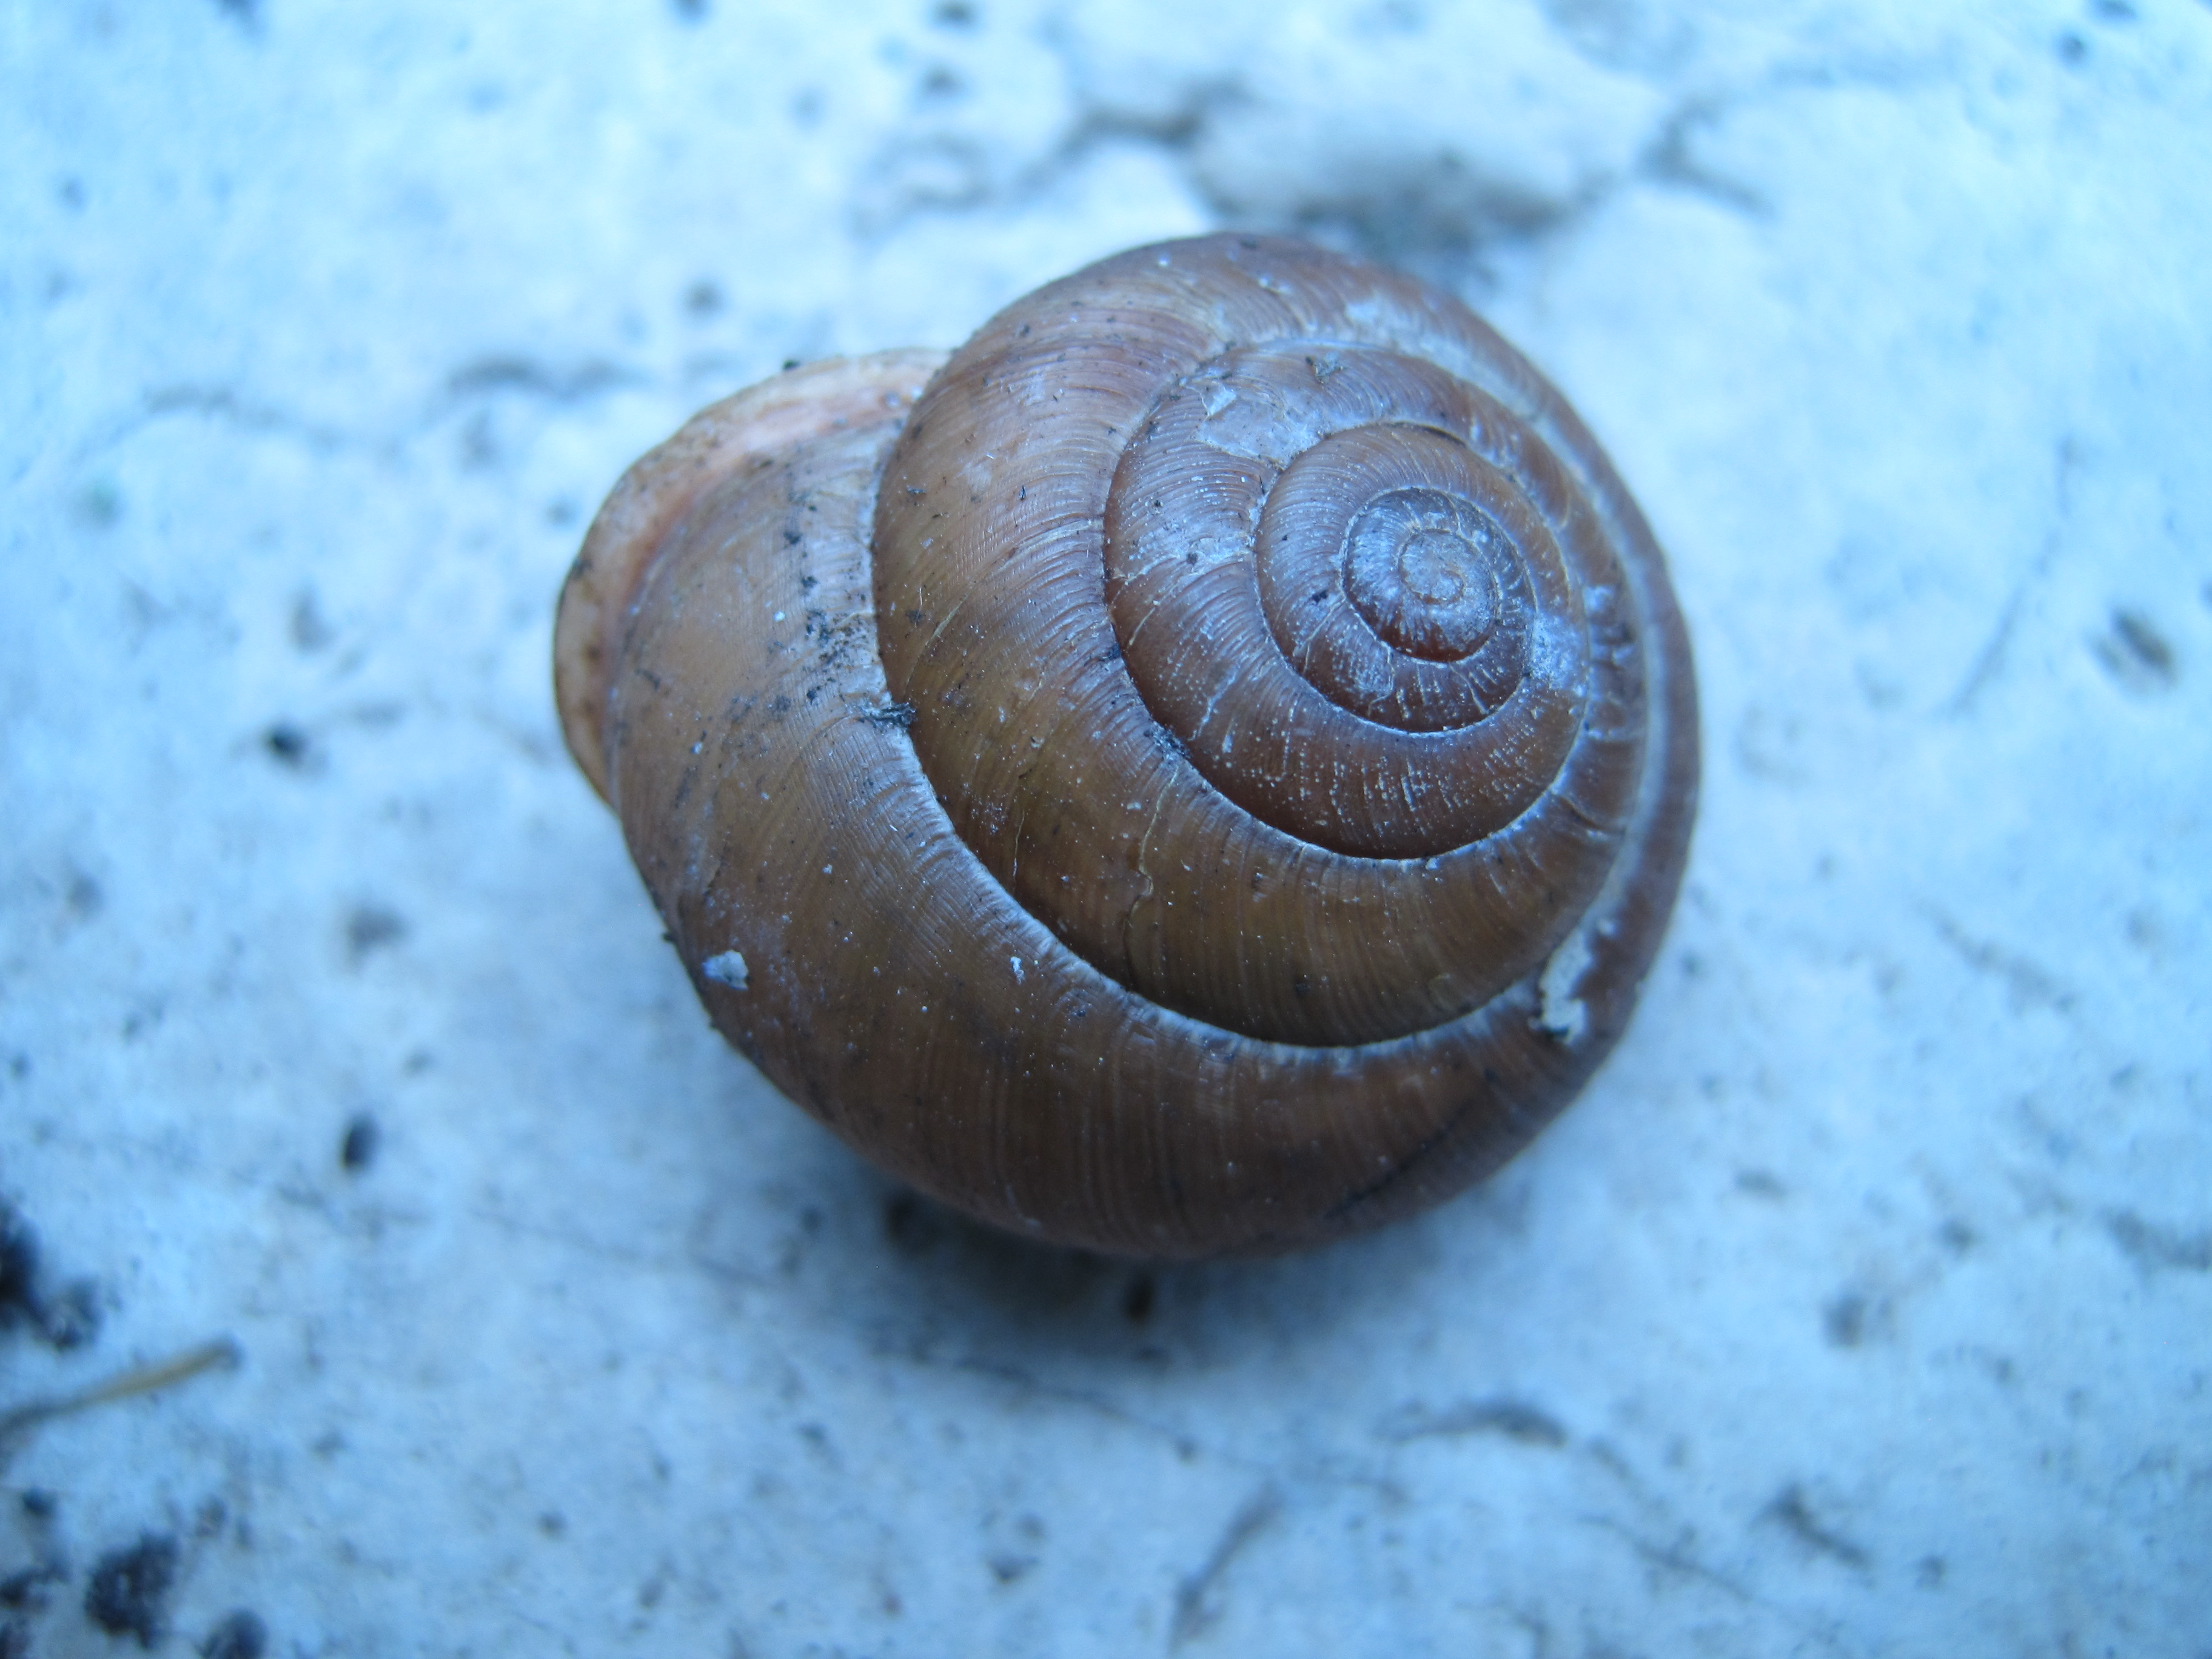
\includegraphics[width=\photosize]{shell}}
        
        \uncover<6->{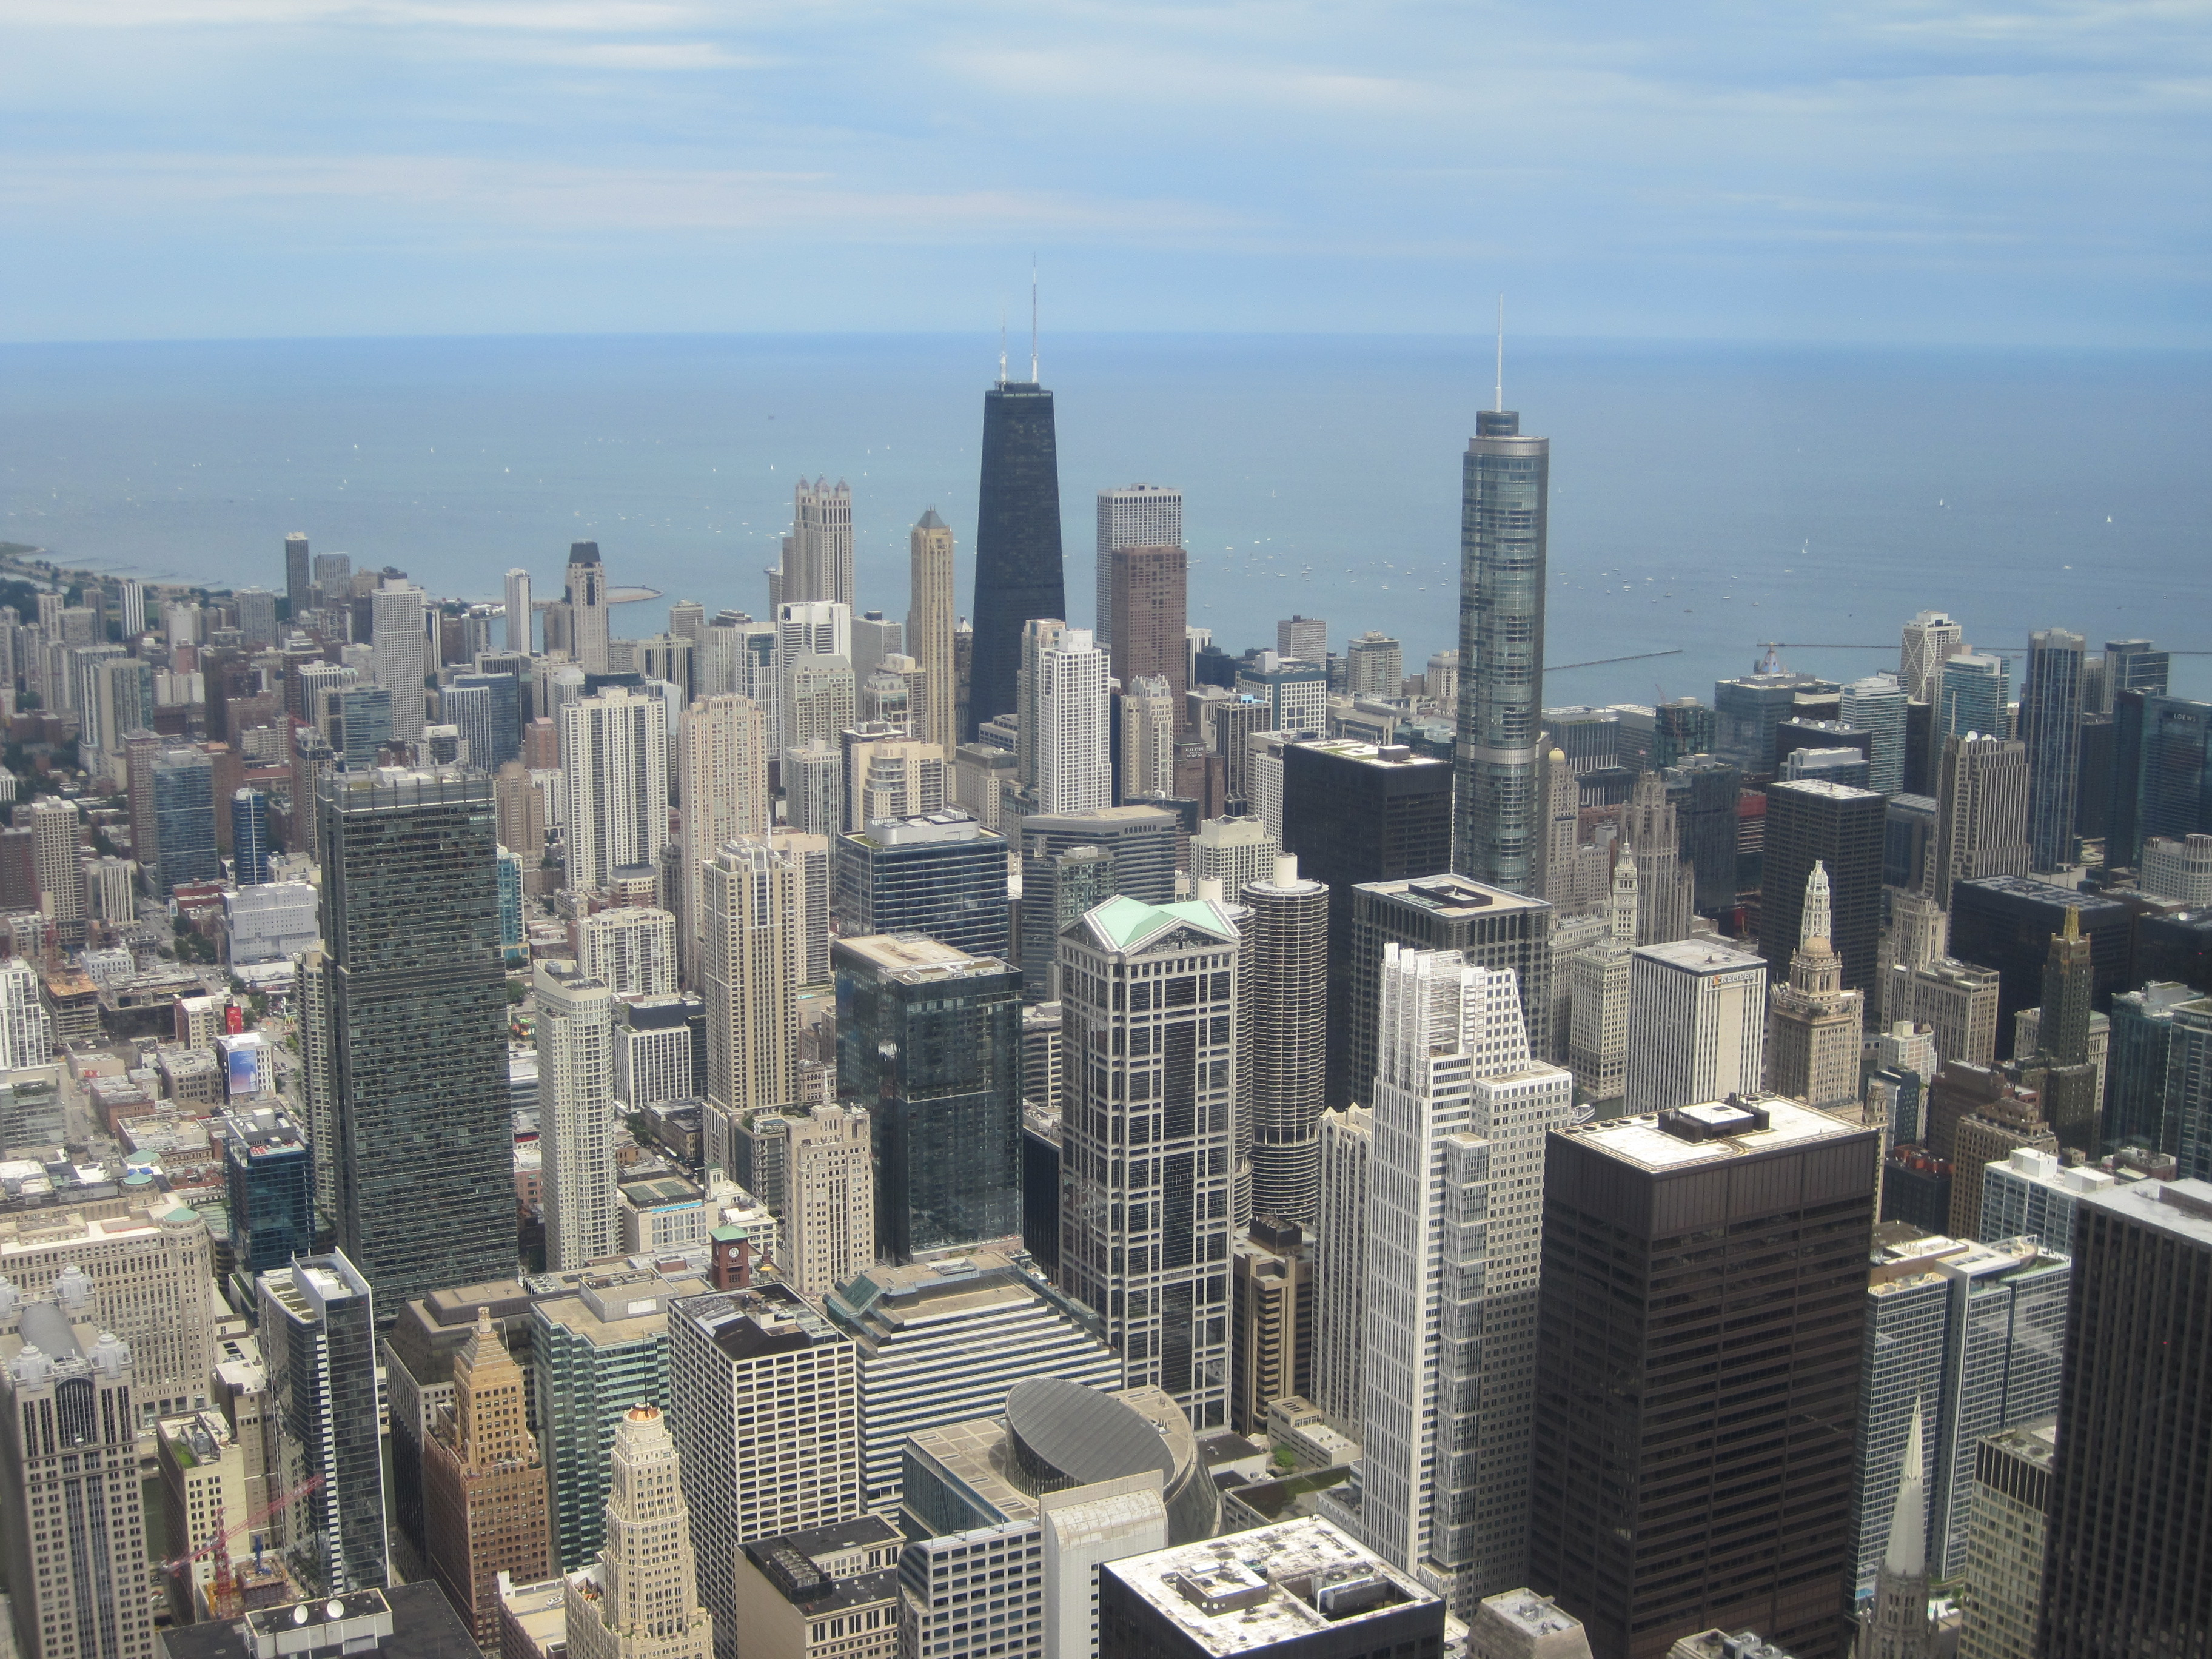
\includegraphics[width=\photosize]{skyline}}
      \end{center}
    \end{column}
  \end{columns}
\end{frame}

\begin{frame}
  \newcommand{\photosize}{0.4\textwidth}

  \frametitle<1-10>{Photo Versions}

  \begin{columns}
    \begin{column}{0.5\textwidth}
      \textbf{Server}
      \only<1-5>{
        \uncover<2->{
          \begin{itemize}
          \item Add 2 images
          \item<3-> Add \texttt{merchmart}
          \end{itemize}
        }
      }
      \only<6->{
        \uncover<7->{
          \begin{itemize}
          \item Add 3 images
          \item<9-> \alert<9>{Remove \texttt{merchmart}}
          \end{itemize}
        }
      }
      \begin{center}
        \uncover<1-9>{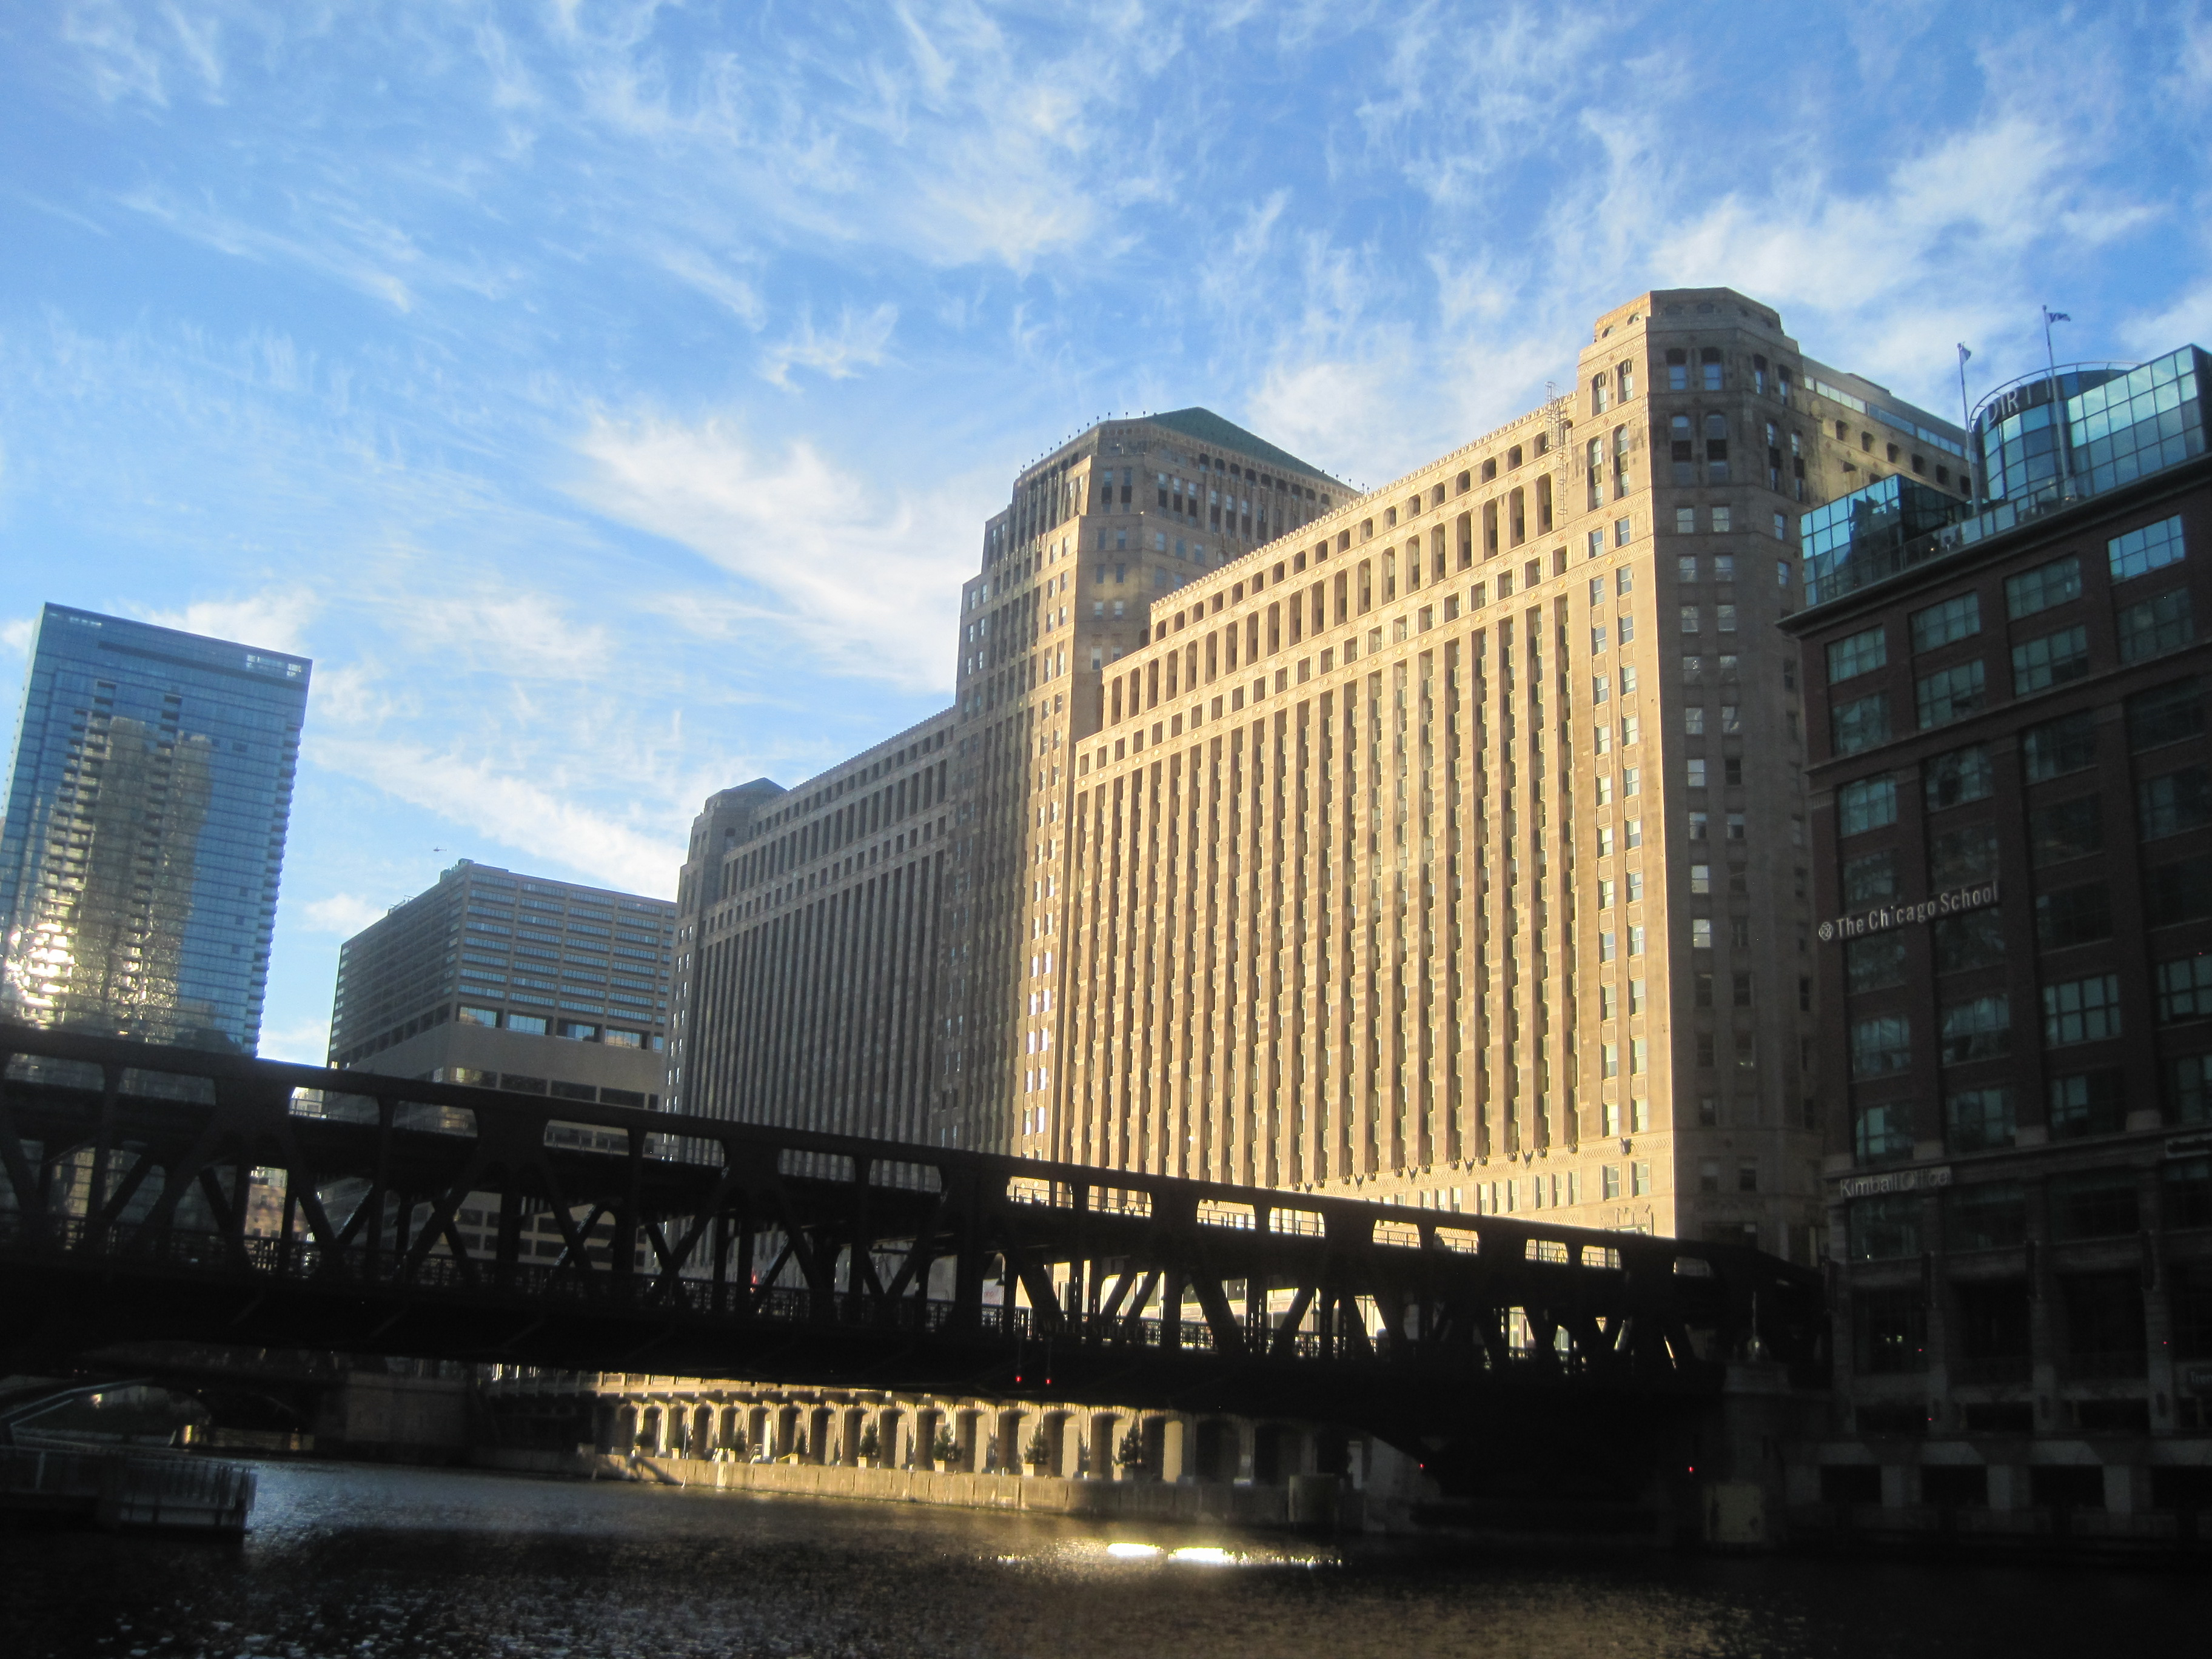
\includegraphics[width=\photosize]{merchmart}}
        
        \uncover<1->{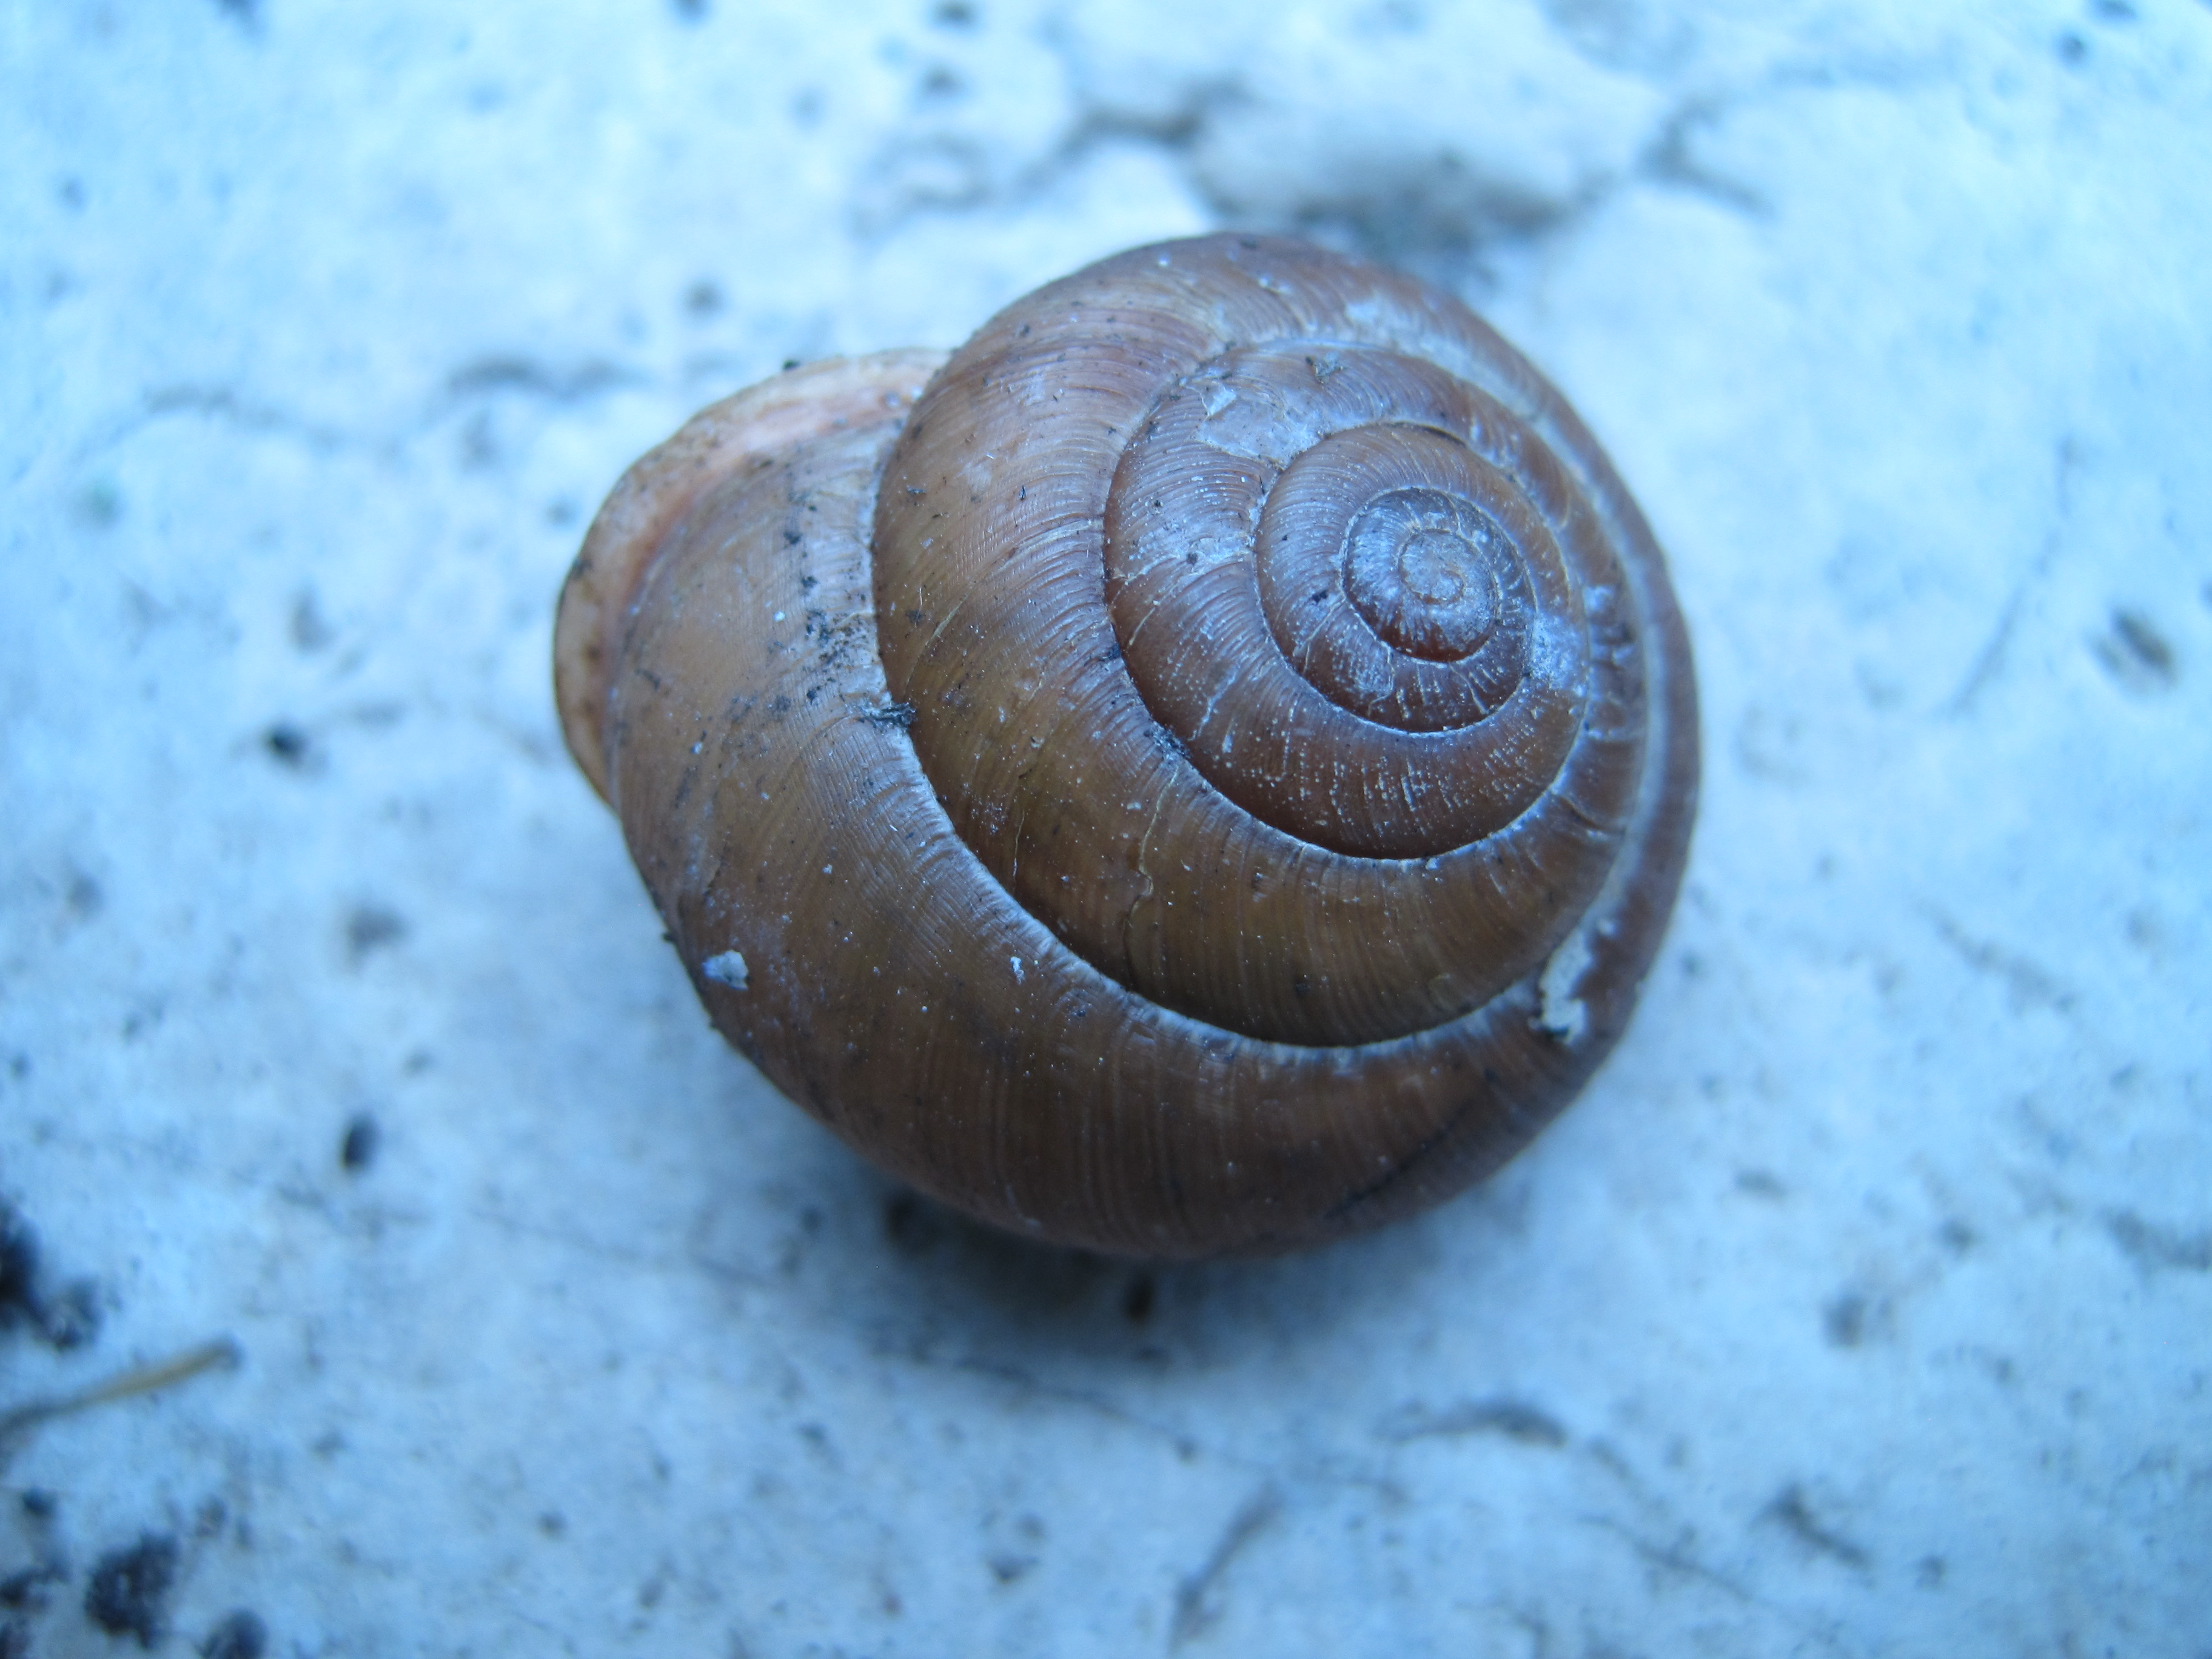
\includegraphics[width=\photosize]{shell}}
        
        \uncover<1->{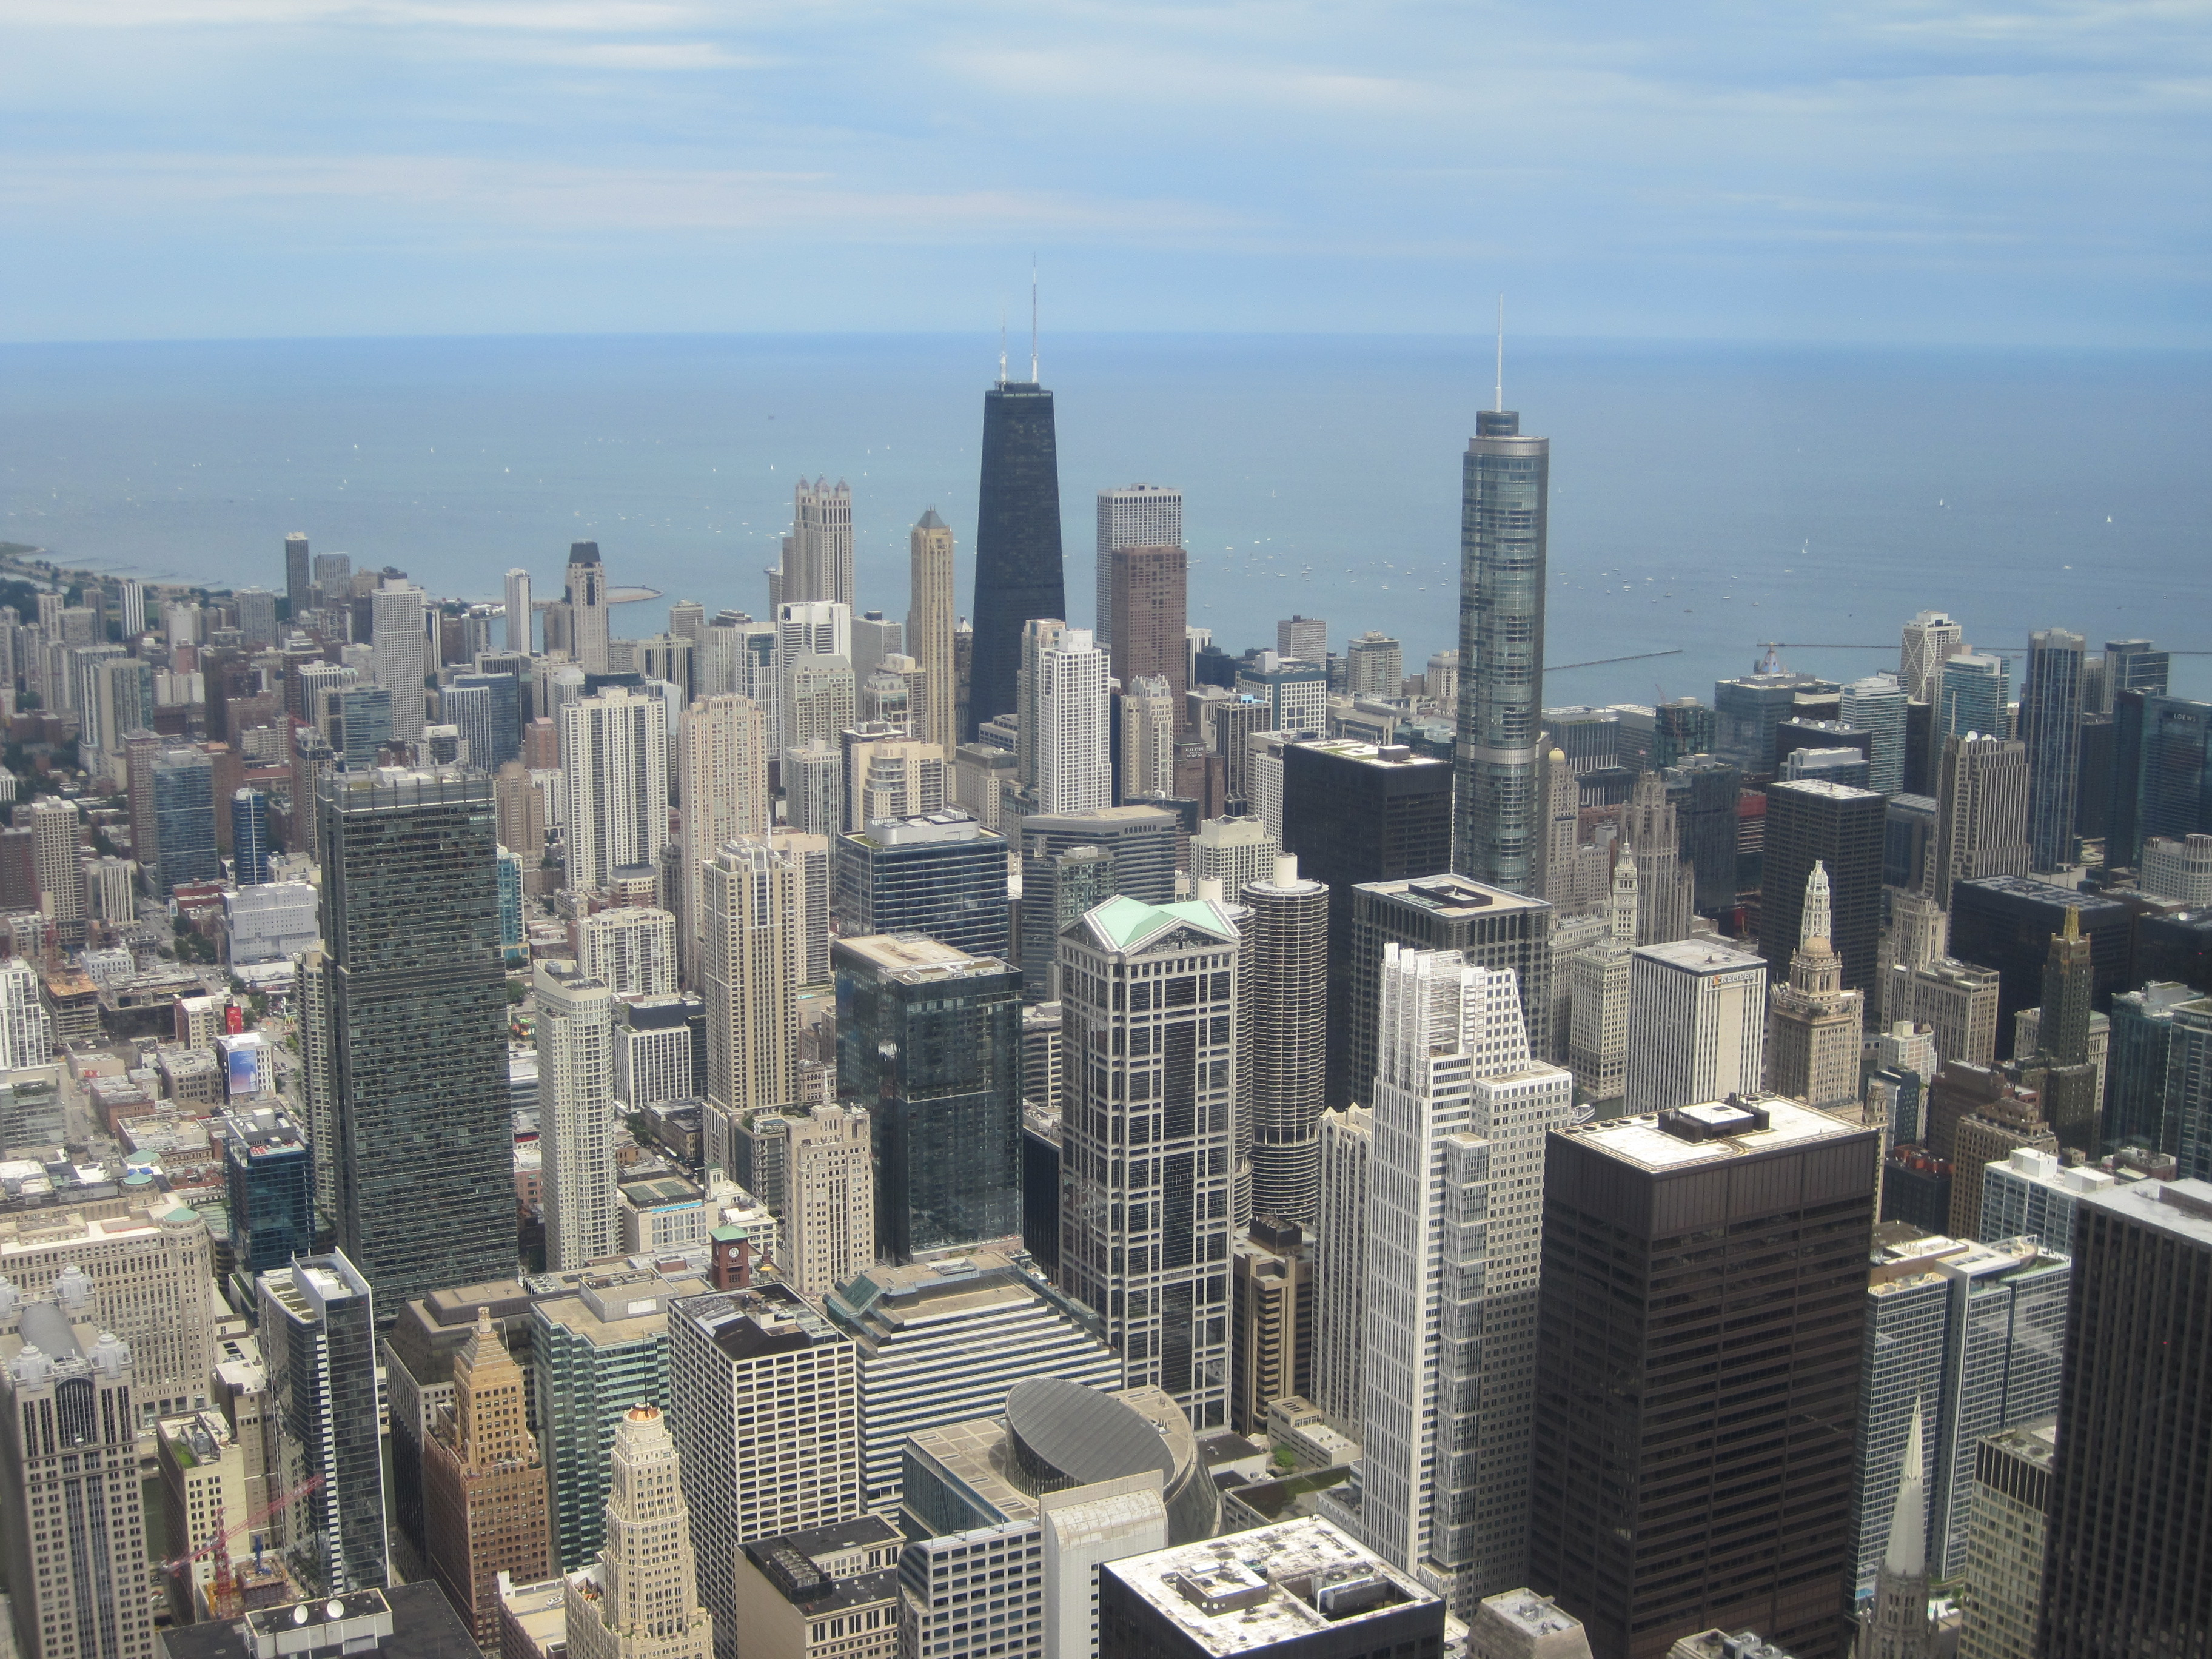
\includegraphics[width=\photosize]{skyline}}
      \end{center}
    \end{column}

    \begin{column}{0.5\textwidth}
      \textbf{Laptop}
      \only<1-5>{
        \uncover<2->{
          \begin{itemize}
          \item Add 2 images
          \item<4-> \alert<4>{Add \texttt{merchmart}}
          \end{itemize}
        }
      }
      \only<6->{
        \uncover<7->{
          \begin{itemize}
          \item Add 3 images
          \item<8-> Remove \texttt{merchmart}
          \end{itemize}
        }
      }
      \begin{center}
        \uncover<5>{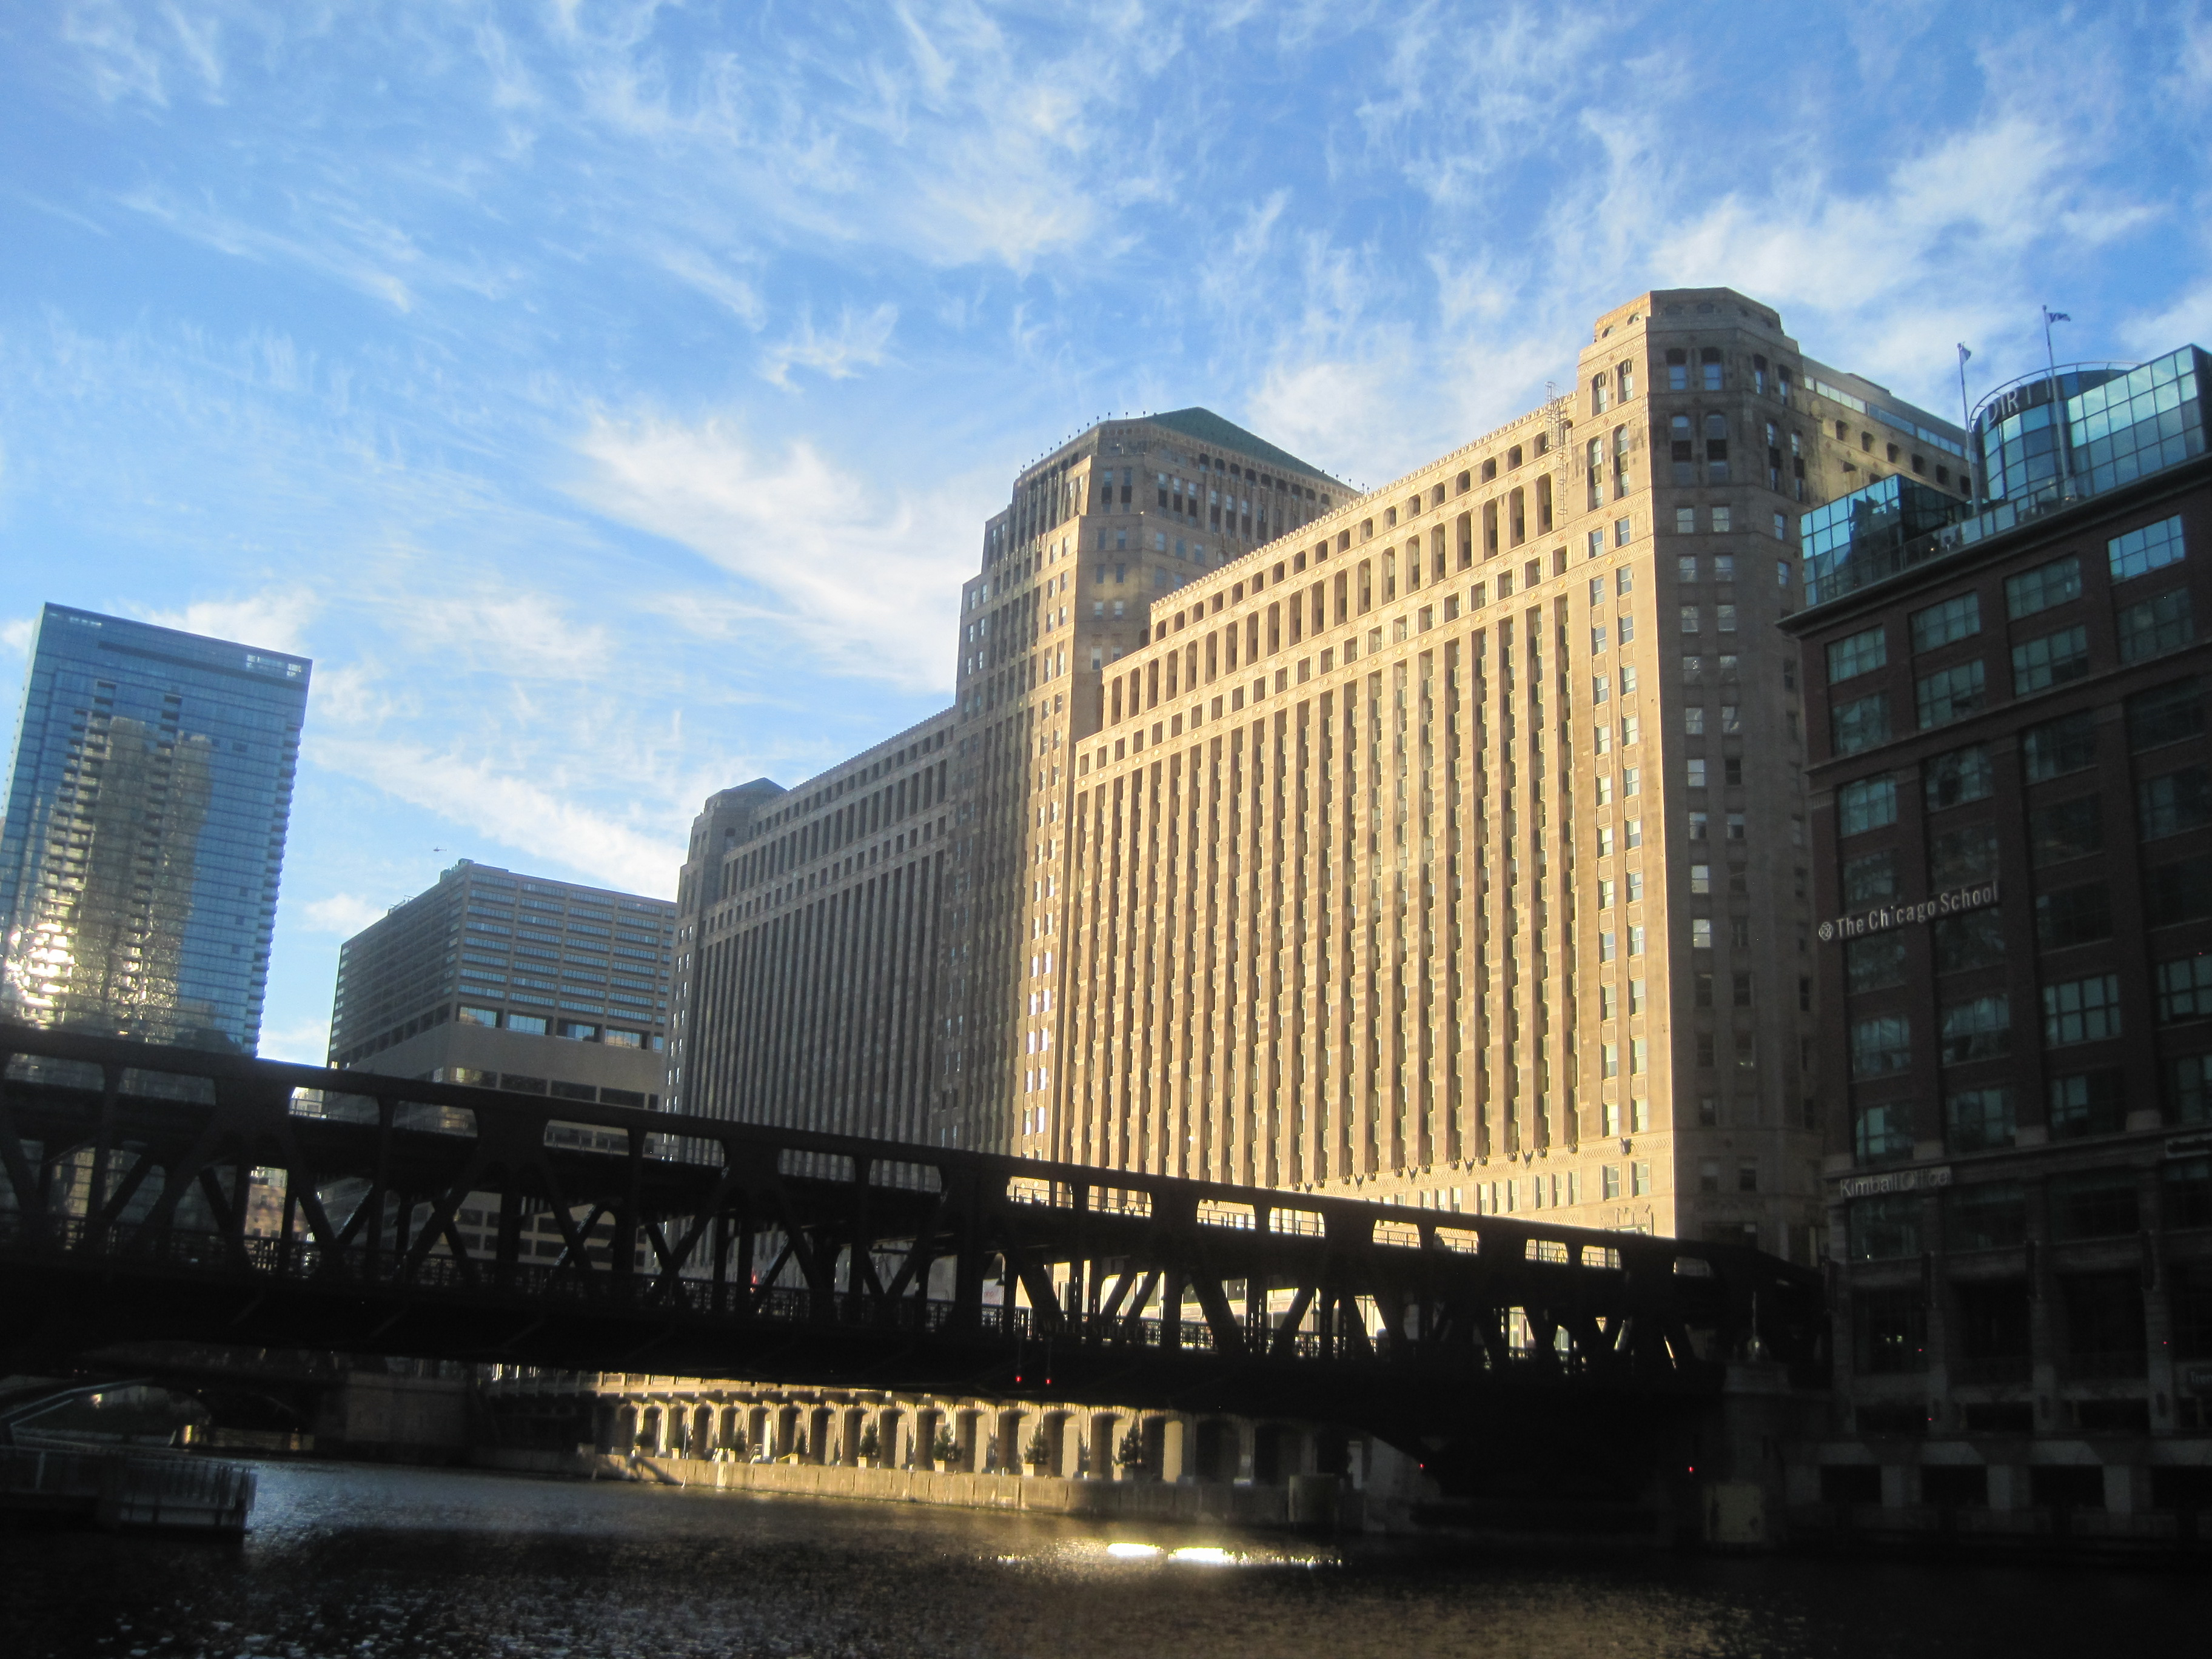
\includegraphics[width=\photosize]{merchmart}}
        
        \uncover<1->{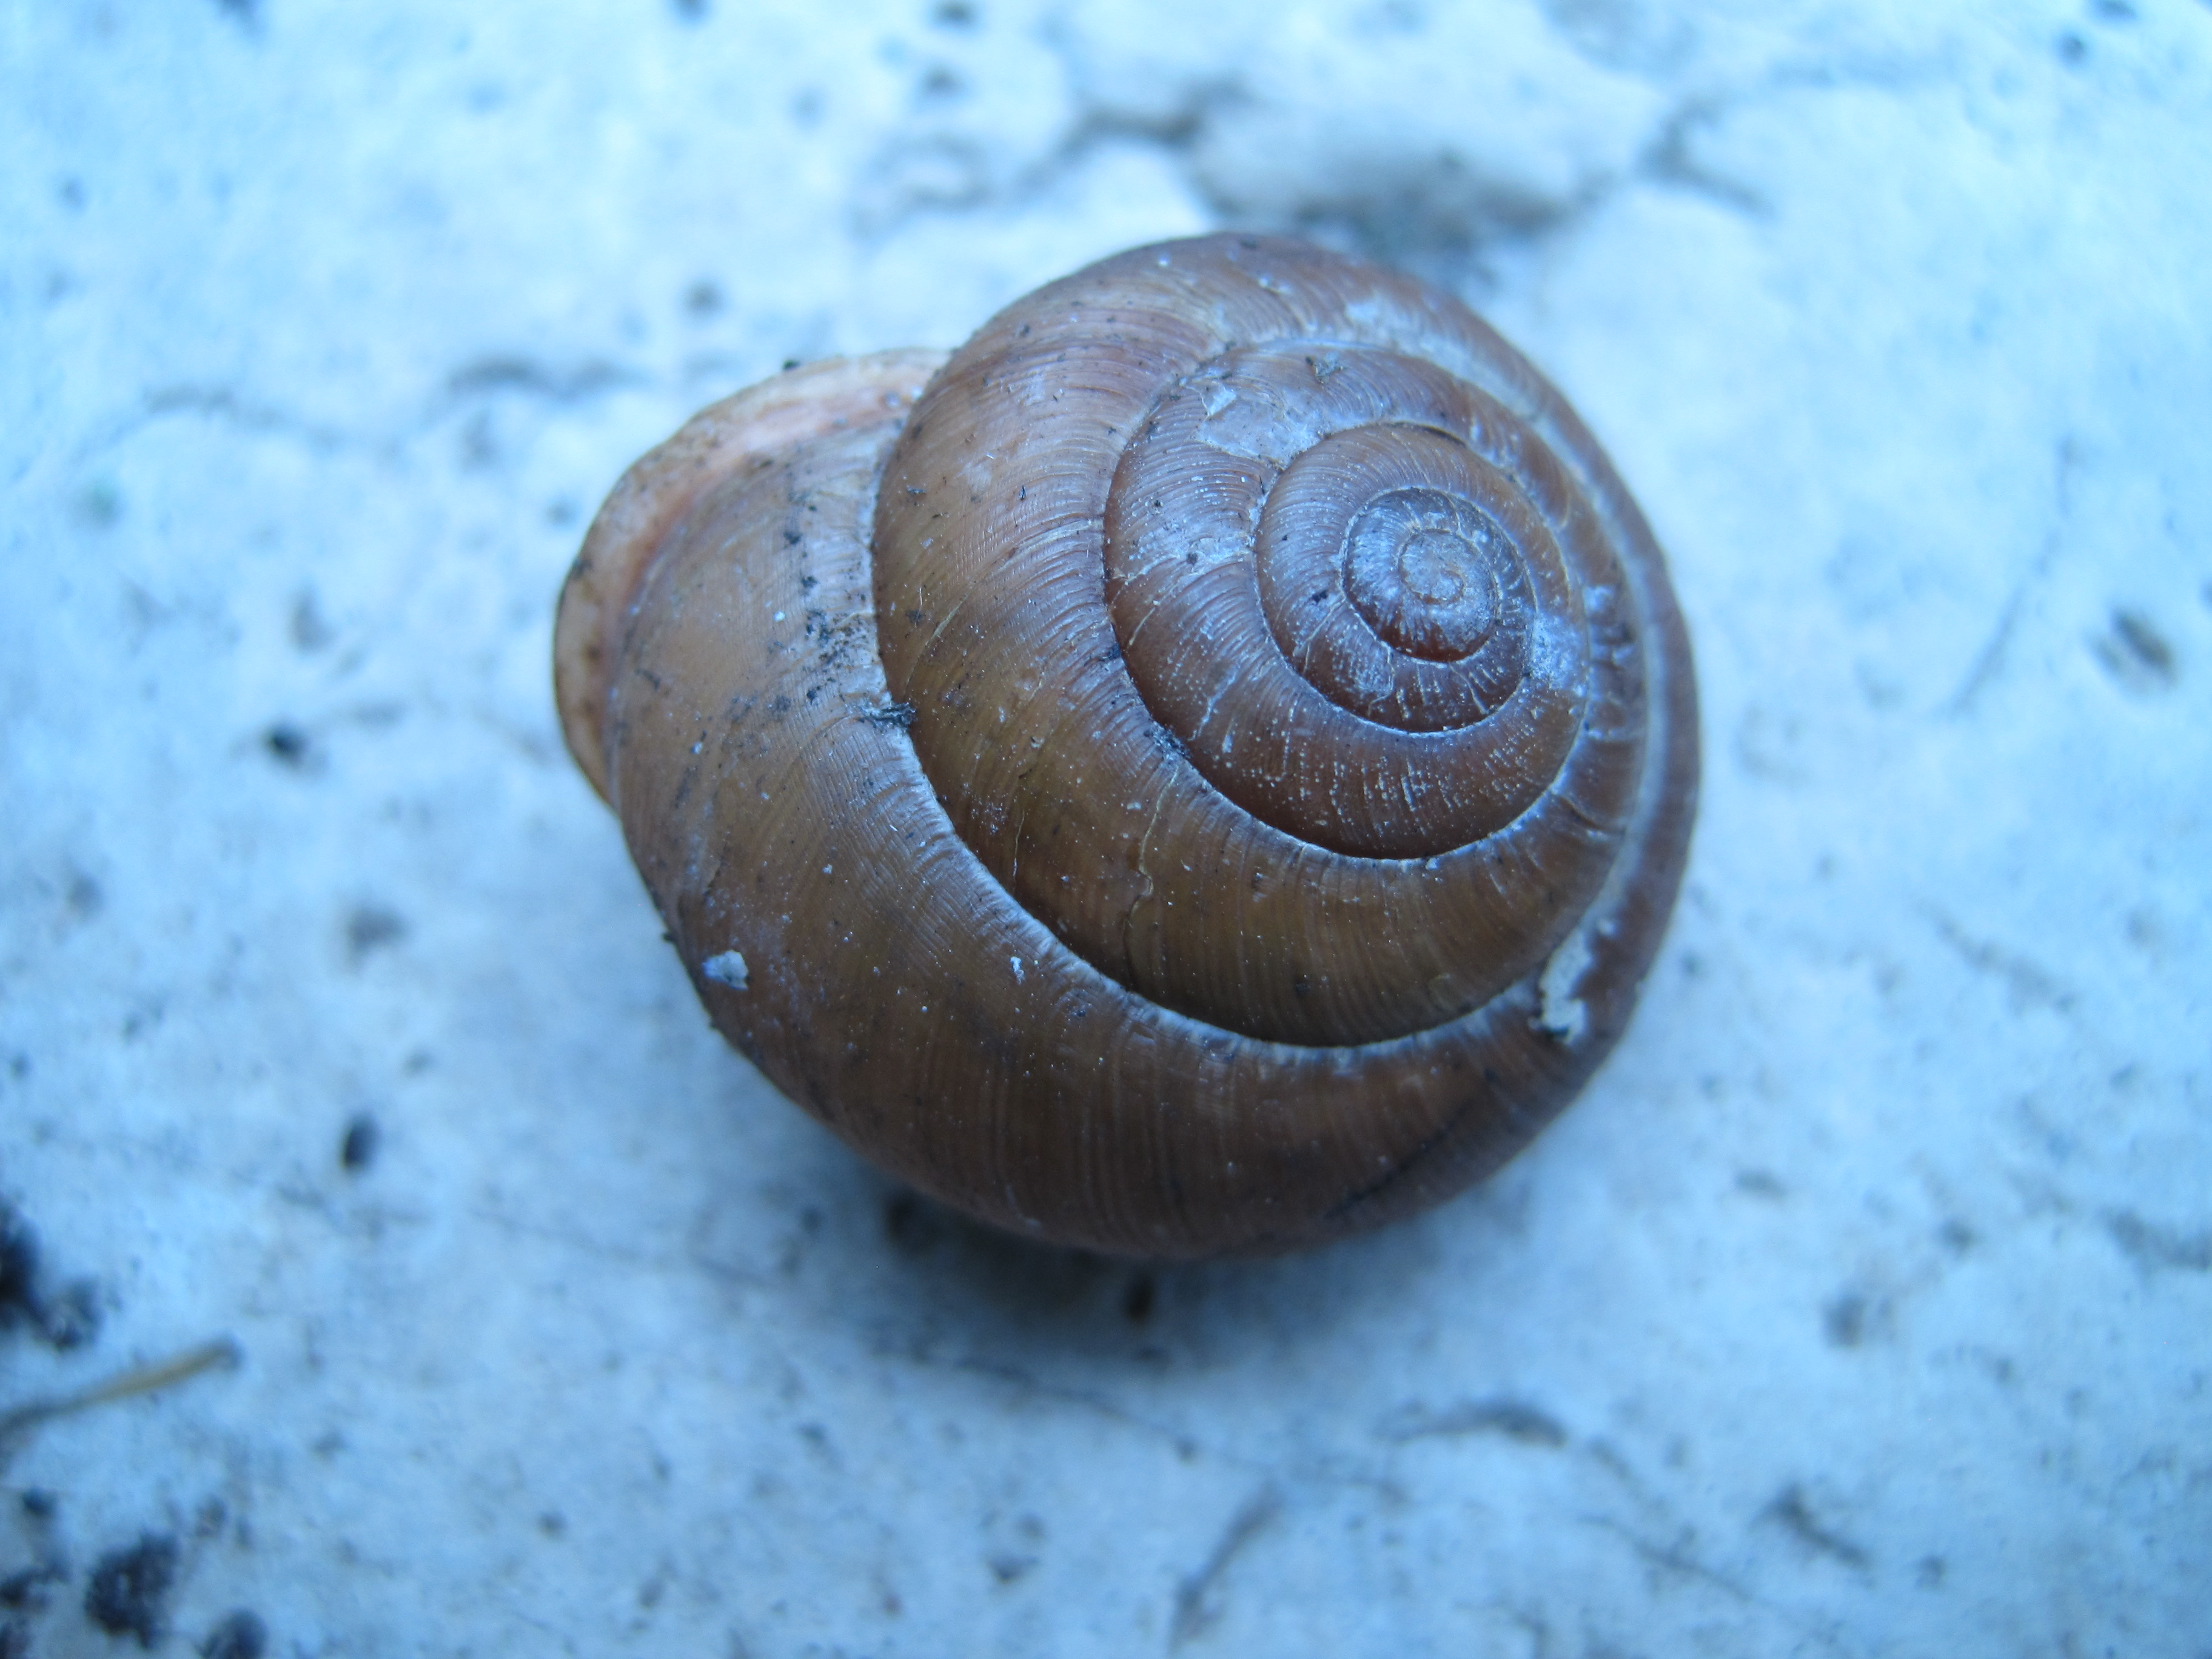
\includegraphics[width=\photosize]{shell}}
        
        \uncover<1->{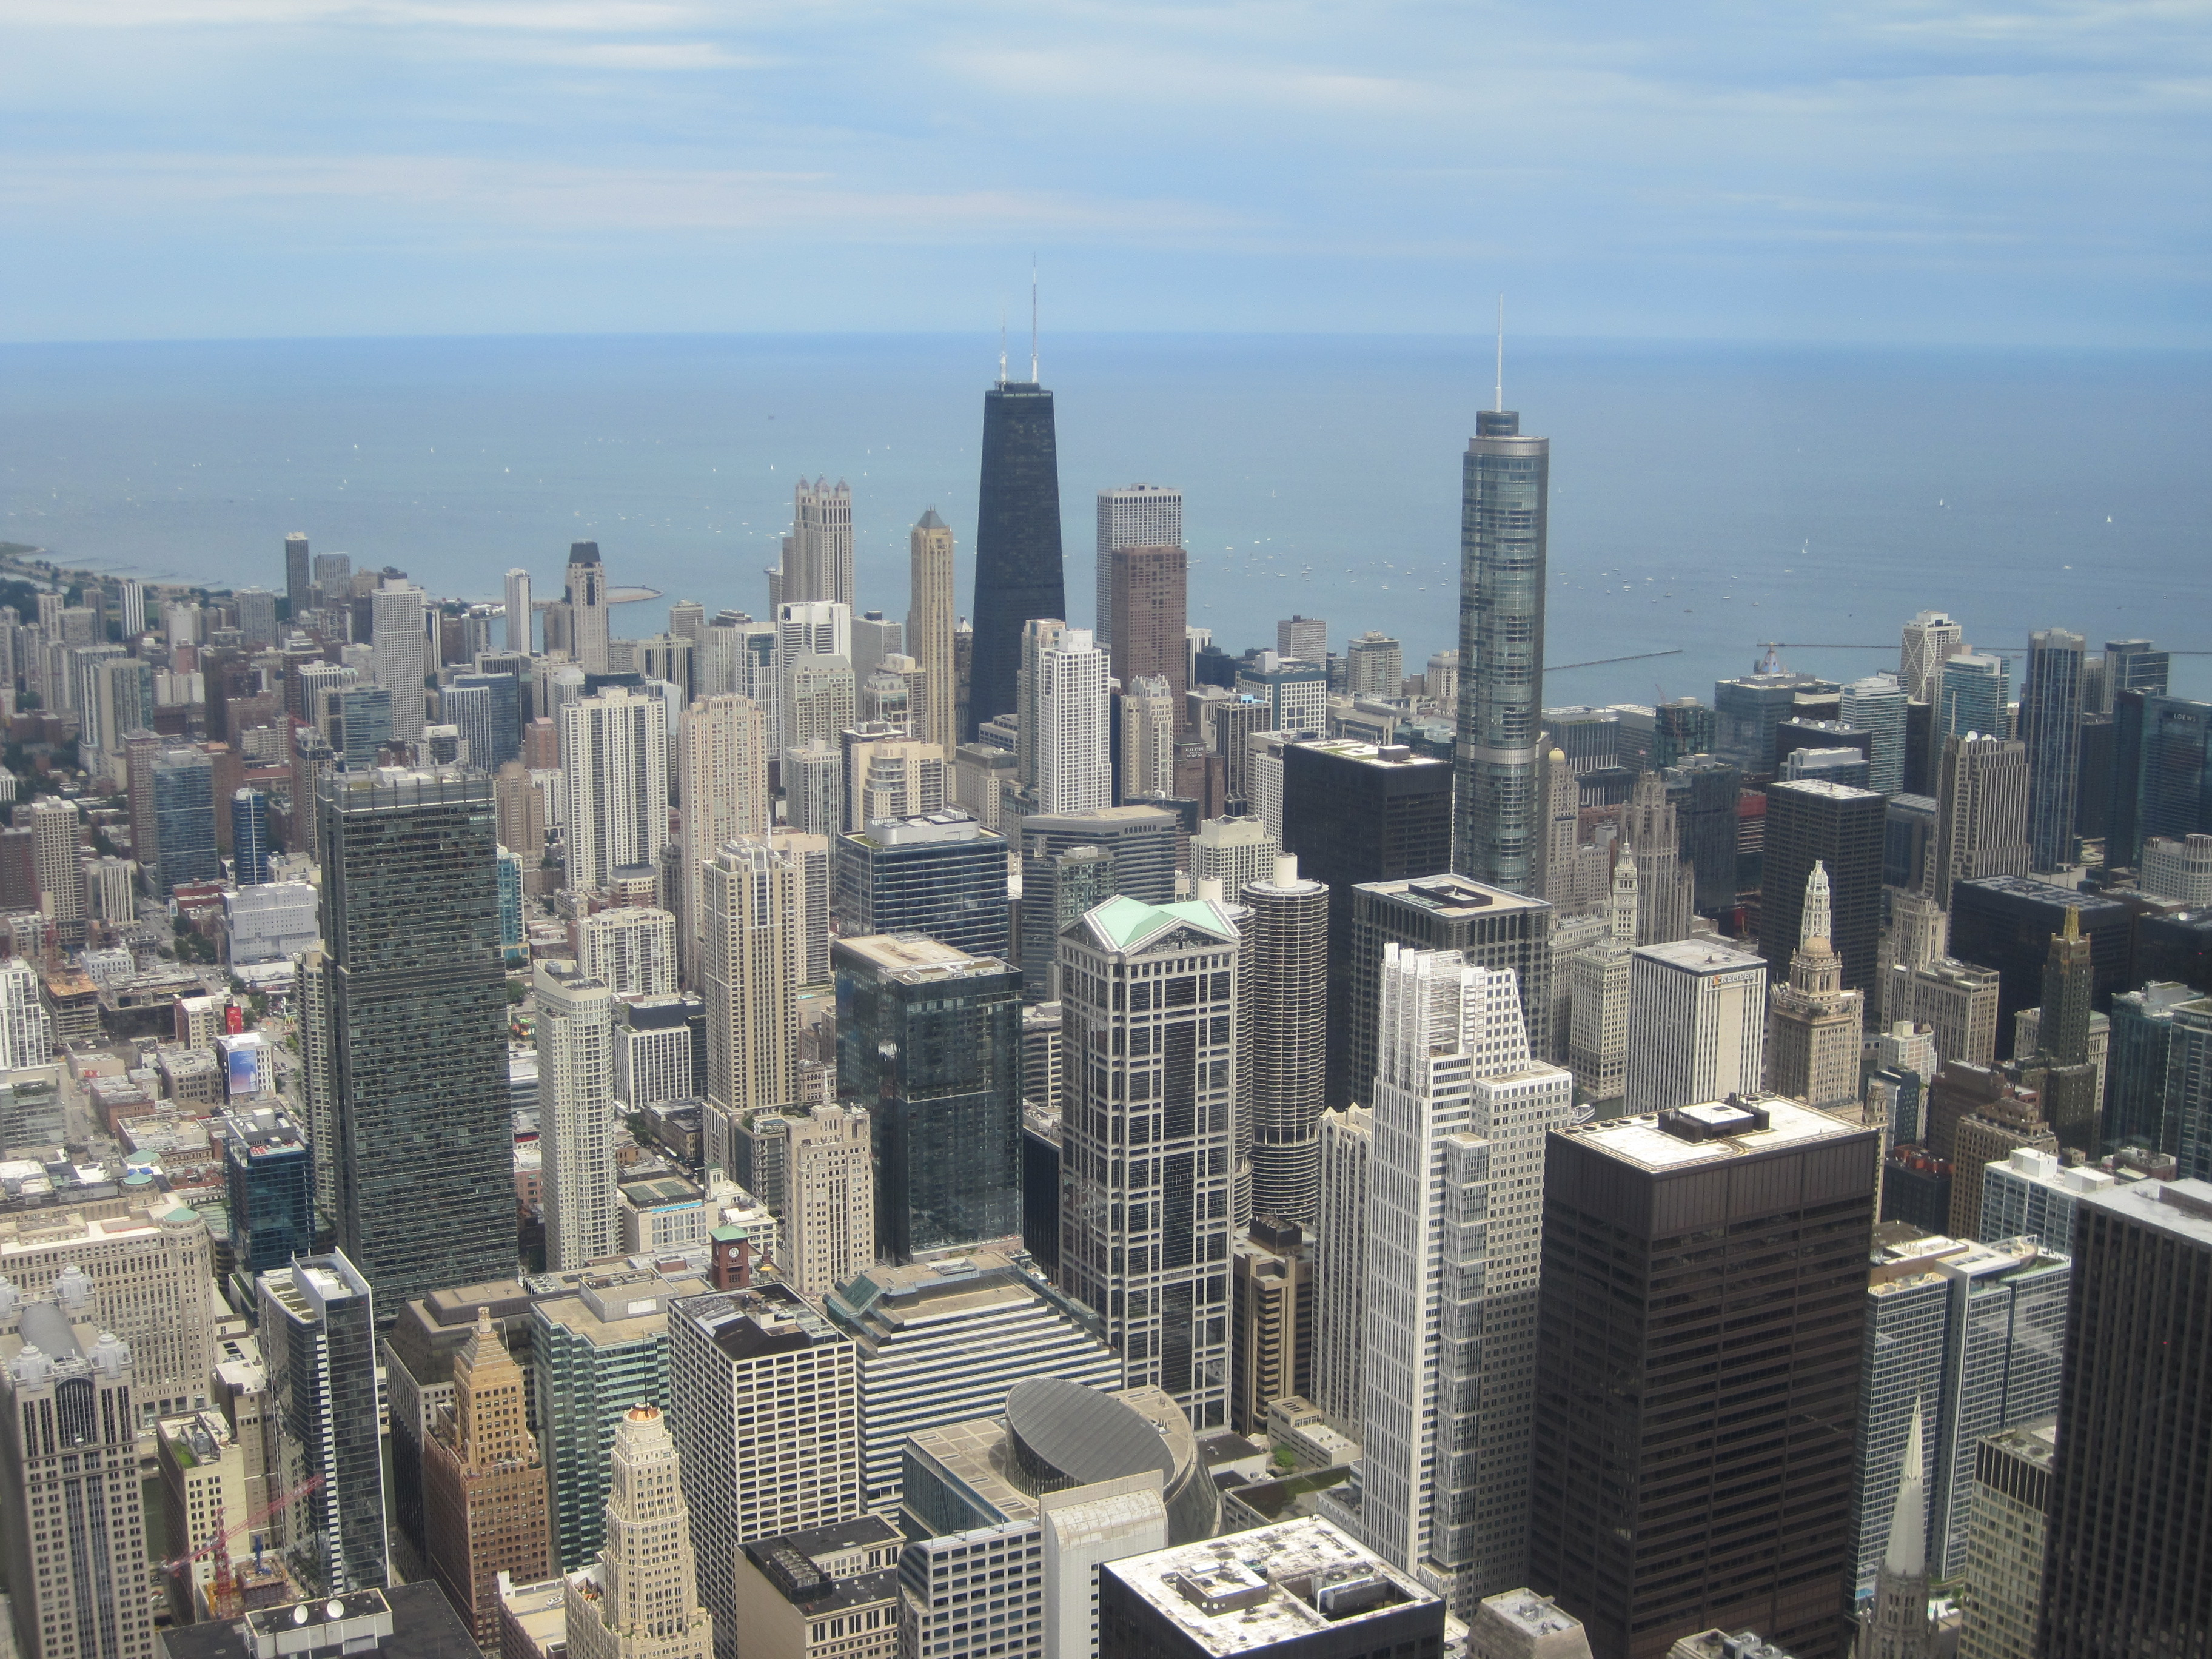
\includegraphics[width=\photosize]{skyline}}
      \end{center}
    \end{column}
  \end{columns}
\end{frame}

\section{Commits}

\subsection{Basics}

\begin{frame}
  \frametitle{What is a Commit?}

  \begin{itemize}
    \pause
  \item A commit fills in the sentence ``Apply \textbf{these changes} to \textbf{this universe} (and some \textbf{other stuff})''
    \begin{itemize}
      \pause
    \item \textbf{``these changes''}: The diff
      \pause
    \item \textbf{``this universe''}: Parent commit
      \pause
    \item \textbf{``other stuff''}: Metadata, like author, timestamp, and commit message
    \end{itemize}
    \pause
  \item Those attributes get combined and run through a hash (I think SHA1) to produce a unique ID
    \pause
  \item Those ID's are the commit SHA that you see everywhere
    \pause
  \item Something like \texttt{a8808ba20c1d3d3f26f685d71a29de3e452d82711}
    \pause
  \item The first 7 of that is almost always unique within a project (\texttt{a8808ba})
  \end{itemize}
\end{frame}

\newcommand{\commit}[3]{
  \node[circle, draw, radius=0.5cm, fill=green](#1) at #2{\texttt{#3}};
}
\newcommand{\selectedcommit}[3]{
  \node[circle, draw, radius=0.5cm, fill=green, thick](#1) at #2{\texttt{#3}};
}
\newcommand{\pendingcommit}[3]{
  \node[circle, draw, radius=0.5cm, fill=yellow](#1) at #2{\textcolor{yellow}{\texttt{#3}}};
}
\newcommand{\textbox}[3]{
  \node(#1)[draw, fill=white, rounded corners, align=left] at #2 {#3};
}

\begin{frame}
  \begin{center}
    \begin{tikzpicture}
      \uncover<8-12, 15-26, 31->{\commit{commit1}{(-3, 0)}{fe4a89}}
      \uncover<4-7, 13-14, 27-30>{\selectedcommit{}{(-3, 0)}{fe4a89}}
      
      \uncover<13-14, 21-27, 34->{\commit{commit2}{(0, 0)}{5768a9}}
      \uncover<8-12, 15-20>{\selectedcommit{}{(0, 0)}{5768a9}}
      \uncover<8-27, 34->{\draw (commit1) -- (commit2);}

      \uncover<21-26, 34->{\selectedcommit{commit3}{(3, 0)}{946efa}}
      \uncover<27>{\commit{}{(3, 0)}{946efa}}
      \uncover<21-27, 34->{\draw (commit2) -- (commit3);}
      
      \uncover<31-33>{\selectedcommit{commit4}{(0, 0)}{43390c}}
      \uncover<31-33>{\draw (commit1) -- (commit4);}

      \uncover<2->{
        \textbox{file}{(-3, -3)}{
          \texttt{\scriptsize \uncover<1-20, 27-30>{\color<20, 30>{gray}{\alt<20, 30>{\sout}{}{There once was a walrus named Joe}}}}\\
          \texttt{\scriptsize Who acted like he did not know}\\
          \texttt{\scriptsize \uncover<7-12, 15-26, 34->{\color<7>{gray}{That he wasn't in a limerick}}}
        }
      }
      
      \uncover<18>{
        \textbox{diff2}{(3, -3)}{
          \texttt{\scriptsize \textcolor{gray}{\ \ There once was a walrus named Joe}}\\
          \texttt{\scriptsize \textcolor{gray}{\ \ Who acted like he did not know}}\\
          \texttt{\scriptsize \textcolor{green}{+ That he wasn't in a limerick}}
        }

        \draw[dashed] (commit2) -- (diff2);
      }

      \uncover<24->{
        \textbox{diff3}{(3, -3)}{
          \texttt{\scriptsize \textcolor{red}{- There once was a walrus named Joe}}\\
          \texttt{\scriptsize \uncover<24-25, 32->{\textcolor{gray}{\ \ Who acted like he did not know}}}\\
          \texttt{\scriptsize \uncover<24-25, 34->{\textcolor{gray}{\ \ That he wasn't in a limerick}}}
        }

        \uncover<24-25, 34->{\draw[dashed] (commit3) -- (diff3);}
        \uncover<32-33>{\draw[dashed] (commit4) -- (diff3);}
      }

      \uncover<1-2>{\textbox{}{(0, 2)}{The word ``commit'' often refers to\\ the state of the world at some point}}
      \uncover<5>{\textbox{}{(0, 2)}{\texttt{fe4a89} is the commit where the file looks like this}}
      \uncover<9>{\textbox{}{(0, 2)}{\texttt{5768a9} is the commit where the file looks like this}}
      \uncover<11-15>{\textbox{}{(0, 2)}{Navigate between commits with \texttt{git checkout <SHA>}}}
      \uncover<12>{\textbox{}{(0, -1.5)}{\texttt{git checkout fe4a89}}}
      \uncover<14>{\textbox{}{(0, -1.5)}{\texttt{git checkout 5768a9}}}
      \uncover<17-18>{\textbox{}{(0, 2)}{The word ``commit'' \textit{also} often refers to\\ the changes between one state and another}}
      \uncover<22>{\textbox{}{(0, 2)}{\texttt{946efa} is the commit where the file looks like this}}
      \uncover<25>{\textbox{}{(0, 2)}{\texttt{946efa} is \textit{also} this change, applied to \texttt{5768a9}}}
      \uncover<29-32>{\textbox{}{(0, 2)}{The same changes applied to \texttt{fe4a89}\\ would be a different commit}}
      \uncover<33->{\textbox{}{(0, 2)}{Different from \texttt{946efa} earlier}}
    \end{tikzpicture}
  \end{center}
\end{frame}

\begin{frame}
  \begin{itemize}
    \pause
  \item Git is not ultimately about history.
    \pause
  \item Git is about revealing \textit{intention}.
    \pause
  \item History and commits are a tool for revealing the intention behind discrepancies.
    \begin{itemize}
      \pause
    \item Did I intend to delete the photo here?
      \pause
    \item ...or did I want to add it there?
    \end{itemize}
    \pause
  \item We will revisit this theme of intentions many times.
  \end{itemize}
\end{frame}

\subsection{Refspecs}

\newcommand{\squiggle}{\~{}}

\begin{frame}
  \frametitle{Refspecs}

  \begin{itemize}
  \item<2-> A \textbf{refspec} is anything that uniquely identifies a commit.
  \item<3-> The short SHA, like \texttt{946efa} is a refspec.
  \item<4-> A long SHA, like \texttt{946efaa7d9695251a363d4c6fdcb631fcd3d8feed} is too.
  \item<5-> \texttt{HEAD} is a refspec referring to the commit that is currently checked out.
  \item<6-> Adding \texttt{\squiggle} to a refspec refers to that refspec's parent.
  \item<7-> You can get the $n$'th parent (parent-of-a-parent-of-a\ldots) by appending \texttt{\squiggle n} (so the parent of the parent of the parent would be \texttt{\squiggle 3})
  \end{itemize}
\end{frame}

\begin{frame}
  \frametitle{Refspec Examples}

  \begin{center}
    \begin{tikzpicture}
      \uncover<2->{\commit{commit1}{(-3, 0)}{fe4a89}}
     
      \uncover<2->{\commit{commit2}{(0, 0)}{5768a9}}
      \uncover<2->{\draw (commit1) -- (commit2);}
      
      \uncover<2->{\selectedcommit{commit3}{(3, 0)}{946efa}}
      \uncover<2->{\draw (commit2) -- (commit3);}
    \end{tikzpicture}
  \end{center}

  \begin{itemize}
  \item<3-> \texttt{946efa} and \texttt{HEAD} refer to the same commit.
  \item<4-> \texttt{HEAD\squiggle } and \texttt{946efa\squiggle } both refer to \texttt{5768a9}.
  \item<5-> \texttt{fe4a89} could be identified by any of: \texttt{5768a9\squiggle }, \texttt{946efa\squiggle \squiggle }, \texttt{946efa\squiggle 2}, \texttt{HEAD\squiggle \squiggle }, or \texttt{HEAD\squiggle 2}
  \end{itemize}
\end{frame}

\begin{frame}
  \begin{itemize}
  \item<1-> \alert{Refspecs are not immutable.}
  \item<2-> Some, like the SHA's, are.
    \begin{itemize}
    \item<3-> \texttt{946efa} will always refer to that specific commit.
    \end{itemize}
  \item<4-> Others, like \texttt{HEAD}, are not.
    \begin{itemize}
    \item<5-> If you \texttt{git checkout} a different commit, \texttt{HEAD} will refer to \textit{that} commit afterwards.
    \end{itemize}
  \item<6-> (Spoilers) Branches are intended to be mutable. Tags are intended to be immutable, but can be changed in a pinch.
  \end{itemize}
\end{frame}

\subsection{Branching and Merging}

\begin{frame}
  \frametitle{Why Branching?}
  
  \begin{itemize}
    \pause
  \item Typically, the ``source of truth'' version of code that everyone can agree on is on a branch called \texttt{master}.
    \pause
  \item It's useful to track changes on work that hasn't been agreed on yet.
  \end{itemize}
\end{frame}

\newcommand{\anoncommit}[2]{
  \node[circle, draw, minimum size=1cm, fill=green](#1) at #2{};
}
\newcommand{\selectedanoncommit}[2]{
  \node[circle, draw, minimum size=1cm, fill=green, thick](#1) at #2{};
}
\newcommand{\branch}[3]{
  \node[draw, fill=yellow](#1) at #2{\texttt{#3}};
}
\newcommand{\selectedbranch}[3]{
  \node[draw, fill=yellow, thick](#1) at #2{\texttt{#3}};
}

\begin{frame}
  \begin{center}
    \begin{tikzpicture}
      \uncover<1-7, 13-16>{\selectedanoncommit{commit1}{(-3, 0)}}
      \uncover<8-12, 17->{\anoncommit{commit1}{(-3, 0)}}
      
      \uncover<8->{
        \uncover<8>{\selectedanoncommit{commit2}{(0, 0)}}
        \uncover<9->{\anoncommit{commit2}{(0, 0)}}
        \draw (commit1) -- (commit2);
      }

      \uncover<9->{
        \uncover<9-12>{\selectedanoncommit{commit3}{(3, 0)}}
        \uncover<13->{\anoncommit{commit3}{(3, 0)}}
        \draw (commit2) -- (commit3);
      }

      \uncover<17->{
        \selectedanoncommit{commit4}{(-1, 2)}
        \draw (commit1) -- (commit4);
      }

      \uncover<6-7>{
        \selectedbranch{poetry}{(-2, 1.7)}{poetry}
        \draw (poetry) -- (commit1);
      }
      \uncover<8>{
        \selectedbranch{poetry}{(0, 1)}{poetry}
        \draw (poetry) -- (commit2);
      }
      \uncover<9->{
        \uncover<9-12>{\selectedbranch{poetry}{(3, 1)}{poetry}}
        \uncover<13->{\branch{poetry}{(3, 1)}{poetry}}
        \draw (poetry) -- (commit3);
      }
      \uncover<15-16>{
        \selectedbranch{wording}{(-2, 1.7)}{wording}
        \draw (wording) -- (commit1);
      }
      \uncover<17->{
        \selectedbranch{wording}{(-1, 3)}{wording}
        \draw (wording) -- (commit4);
      }
      \uncover<3->{
        \uncover<3-5, 13-14>{\selectedbranch{master}{(-3, 1)}{master}}
        \uncover<6-12, 15->{\branch{master}{(-3, 1)}{master}}
        \draw (master) -- (commit1);
      }

      \uncover<1->{
        \textbox{file}{(0, -2)}{
          \texttt{\scriptsize \uncover<1-8, 13->{There once was a walrus named Joe}}\\
          \texttt{\scriptsize Who acted like he \only<1-16>{{\color<16>{gray}\only<16>{\sout}{did not}}}\only<16>{ }\only<16->{{\color<16>{gray}didn't}} know}\\
          \texttt{\scriptsize \uncover<8-12>{That he wasn't in a limerick}}
        }
      }
      
      \uncover<2-3>{\textbox{}{(0, 4)}{\texttt{master} is the current source of truth}}
      \uncover<4-6>{\textbox{}{(0, 4)}{More work might go onto a different branch}}
      \uncover<7-9>{\textbox{}{(0, 4)}{The checked-out branch advances when you commit}}
      \uncover<11-17>{\textbox{}{(0, 4)}{Multiple branches can have the same branch point}}
      \uncover<19>{\textbox{}{(0, 4)}{\texttt{master} is an ancestor of \texttt{wording}}}
      \uncover<21>{\textbox{}{(0, 4)}{\texttt{master} is also an ancestor of \texttt{poetry}}}
      \uncover<23>{\textbox{}{(0, 4)}{\texttt{poetry} and \texttt{wording} have no ancestry relationship}}
      
      \uncover<5>{\textbox{}{(0, 2.5)}{\texttt{git checkout -b poetry}}}
      \uncover<12>{\textbox{}{(0, 2.5)}{\texttt{git checkout master}}}
      \uncover<14>{\textbox{}{(0, 2.5)}{\texttt{git checkout -b wording}}}
    \end{tikzpicture}
  \end{center}
\end{frame}

\begin{frame}
  \frametitle{Ancestry}
  
  \begin{itemize}
    \pause
  \item Commit $A$ is an \textbf{ancestor} of commit $B$ if $A$ is $B$'s parent, or $B$'s parent's parent, or so on.
    \pause
    \begin{itemize}
      \pause
    \item We might also say that $B$ is \textbf{ahead of} $A$.
    \end{itemize}
  \item This means that there are no changes on $A$ that $B$ doesn't also know about.
    \pause
  \item Commit $A$ being an ancestor of $B$ shows \textit{intention}.
    \begin{itemize}
      \pause
    \item That if there's any question, $B$'s changes are more accurate than $A$'s.
    \end{itemize}
    \pause
  \item Commits without an ancestry relationship leave that intention ambiguous.
    \begin{itemize}
      \pause
    \item We sometimes say that commits with no ancestry relationship have \textbf{diverged}, or are \textbf{divergent}.
    \end{itemize}
  \end{itemize}
\end{frame}

\begin{frame}
  \frametitle{Merging}

  \begin{itemize}
    \pause
  \item Having branches is useful if you have parallel workstreams.
    \begin{itemize}
      \pause
    \item A feature that takes time to implement, compared to a hotfix, for instance.
    \end{itemize}
    \pause
  \item But we need a way to pull those diverging changes back together.
  \end{itemize}
\end{frame}

\begin{frame}
  \begin{center}
    \begin{tikzpicture}
      \anoncommit{commit1}{(-3, 0)}
      
      \anoncommit{commit2}{(0, 0)}
      \draw (commit1) -- (commit2);
      
      \uncover<6-7, 21->{\selectedanoncommit{commit3}{(3, 0)}}
      \uncover<1-5, 8-20>{\anoncommit{commit3}{(3, 0)}}
      \draw (commit2) -- (commit3);
      
      \uncover<1-5, 8-10, 16-17>{\selectedanoncommit{commit4}{(-2, 2)}}
      \uncover<6-7, 11-15, 18->{\anoncommit{commit4}{(-2, 2)}}
      \draw (commit1) -- (commit4);

      \uncover<11->{
        \uncover<11-15, 18-20>{\selectedanoncommit{commit5}{(4, 2)}}
        \uncover<16-17, 21->{\anoncommit{commit5}{(4, 2)}}
        \draw (commit3) -- (commit5);
        \draw (commit4) -- (commit5);
      }
      
      \branch{master}{(-3, 1)}{master}
      \draw (master) -- (commit1);
      
      \uncover<6-7>{\selectedbranch{poetry}{(3, 1)}{poetry}}
      \uncover<1-5, 8->{\branch{poetry}{(3, 1)}{poetry}}
      \draw (poetry) -- (commit3);
      
      \uncover<1-10>{
        \uncover<1-5, 8->{\selectedbranch{wording}{(-2, 3)}{wording}}
        \uncover<6-7>{\branch{wording}{(-2, 3)}{wording}}
        \draw (wording) -- (commit4);
      }
      \uncover<11->{
        \uncover<1-5, 8-15, 18-20>{\selectedbranch{wording}{(4, 3)}{wording}}
        \uncover<6-7, 16-17, 21->{\branch{wording}{(4, 3)}{wording}}
        \draw (wording) -- (commit5);
      }

      \textbox{file}{(0, -2)}{
        \texttt{\scriptsize \uncover<1-5, 8-10, 16-17>{There once was a walrus named Joe}}\\
        \texttt{\scriptsize Who acted like he \only<6-7, 21->{did not}\only<1-5, 8-20>{didn't} know}\\
        \texttt{\scriptsize \uncover<6-7, 11-15, 18->{That he wasn't in a limerick}}
      }
      
      \uncover<2>{\textbox{}{(0, 4)}{\texttt{wording} has the ``did not'' $\rightarrow$ ``didn't'' change}}
      \uncover<4-6>{\textbox{}{(0, 4)}{\texttt{poetry} has the line addition and removal}}
      \uncover<9-11>{\textbox{}{(0, 4)}{Use \texttt{git merge} to pull the changes from \texttt{poetry} into \texttt{wording}}}
      \uncover<13>{\textbox{}{(0, 4)}{This two-parent commit is called a \textbf{merge commit}}}
      \uncover<14-16>{\textbox{}{(0, 4)}{Get its primary parent with \texttt{SHA\^{}1}}}
      \uncover<19->{\textbox{}{(0, 4)}{Get its other parent with \texttt{SHA\^{}2}}}
      
      \uncover<5>{\textbox{}{(0, 2.5)}{\texttt{git checkout poetry}}}
      \uncover<10>{\textbox{}{(0, 2.5)}{\texttt{git merge poetry}}}
      \uncover<15>{\textbox{}{(0, 2.5)}{\texttt{git checkout wording\^{}1}}}
      \uncover<20>{\textbox{}{(0, 2.5)}{\texttt{git checkout wording\^{}2}}}
    \end{tikzpicture}  
  \end{center}
\end{frame}

\begin{frame}
  \frametitle{Conflicts}
  \begin{itemize}
    \pause
  \item Git can \textit{usually} guess how to combine changes from different branches.
    \pause
  \item When it can't, that creates a \textbf{conflict}, which has to be manually resolved.
    \begin{itemize}
      \pause
    \item Usually things like deleting some code in one branch and modifying it in another.
    \end{itemize}
    \pause
  \item Sometimes Git guesses wrong.
    \begin{itemize}
      \pause
    \item For instance, renaming a variable in one branch, while adding usages of it (under the old name) in another.
      \pause
    \item I call this a \textbf{semantic conflict}.
    \end{itemize}
  \item Because of this, merges should \textit{always} involve human intervention and sanity-checking. They \textit{cannot be automated}.
  \end{itemize}
\end{frame}

\subsection{Remotes}

\begin{frame}
  \frametitle{remotes/origin}
  \begin{itemize}
    \pause
  \item The most common git workflow is to \textbf{clone} a remote repository.
    \pause
  \item That means downloading each of the commits from that repository.
  \end{itemize}
\end{frame}

\section{Rewriting History}

\subsection{Why It's Evil}

\subsection{Why It's Awesome}

\section{Specific Worflows}

\subsection{Amend}

\subsection{Rebase}

\subsection{Interactive Rebase}

\subsection{Fixup Commits}

\subsection{Cherry-Pick and Merge Down}

\subsection{Crafting Commits}

\end{document}
